\documentclass[12pt,a4paper]{article}

% Packages
\usepackage{
    amsmath,
    amssymb,
    graphicx,
    titletoc,
    fancyhdr,
    geometry,
    babel,
    xcolor,
    enumerate,
    fix-cm,
    tocbibind,
    listings,
    float,
    enumitem,
    subcaption,
    hyperref
}

% Define colors
\definecolor{vgreen}{RGB}{104,180,104}
\definecolor{vblue}{RGB}{49,49,255}
\definecolor{vorange}{RGB}{255,143,102}

% Listings customization
\renewcommand\lstlistingname{Figura}
\renewcommand\lstlistlistingname{Figura}

\makeatletter
\newcommand*\@lbracket{[}
\newcommand*\@rbracket{]}
\newcommand*\@colon{:}
\newcommand*\colorIndex{%
    \edef\@temp{\the\lst@token}%
    \ifx\@temp\@lbracket \color{black}%
    \else\ifx\@temp\@rbracket \color{black}%
    \else\ifx\@temp\@colon \color{black}%
    \else \color{vorange}%
    \fi\fi\fi
}
\makeatother

% Setup for listings
\lstset{
    captionpos=b,
    belowcaptionskip=\bigskipamount,
    frame=single,
    basicstyle=\small\ttfamily,
    numbers=left,
    numberstyle=\tiny\color{gray},
    xleftmargin=2em,
    framexleftmargin=2em,
    backgroundcolor=\color{vgreen!10},
    stepnumber=1,
    showstringspaces=false,
    keywordstyle=\color{vblue},
    commentstyle=\color{gray},
    stringstyle=\color{vorange},
}

\begin{document}

\begin{titlepage}
    \centering
    
\includegraphics[scale=1]{M2_Modelos_de_Programación/reporte/figuras/Logo_Tec.png}\\
    \vspace{.5cm}
    \bfseries\large Escuela de Ingeniería y Ciencias
        
    \vspace{5cm}
    \centering
    \textbf{\Huge Cómputo en la Nube}
    \vspace{0.5cm}
        
    {\Large Creación de Contenedores de archivos en la Nube}

    \vspace{5cm}
        
    \textbf{\LARGE Armando Bringas Corpus}
        
    \vspace{0.5cm}
        
    {\large A01200230}
        
    \vfill
        
\end{titlepage}

\section{Introducción}

El objetivo de la siguiente práctica consiste en la utilización de dos de los servicios más populares en la nube, Microsoft Azure y Google Cloud, se estarán generando contenedores de archivos en la nube con ambas plataformas. La creación de contenedores es gran utilidad ya que son espacios para el almacenamiento de archivos como imágenes o documentos que se deseen conservar con el tiempo y que sean disponibles a diversos usuarios de forma remota.

\section{Contenedor Azure}

El primer paso es la creación de cuenta de almacenamiento dentro de la plataforma de Microsoft Azure la cual será generada a partir de nuestra cuenta de estudiante que activamos con anterioridad.

\begin{figure}[H]
    \centering
    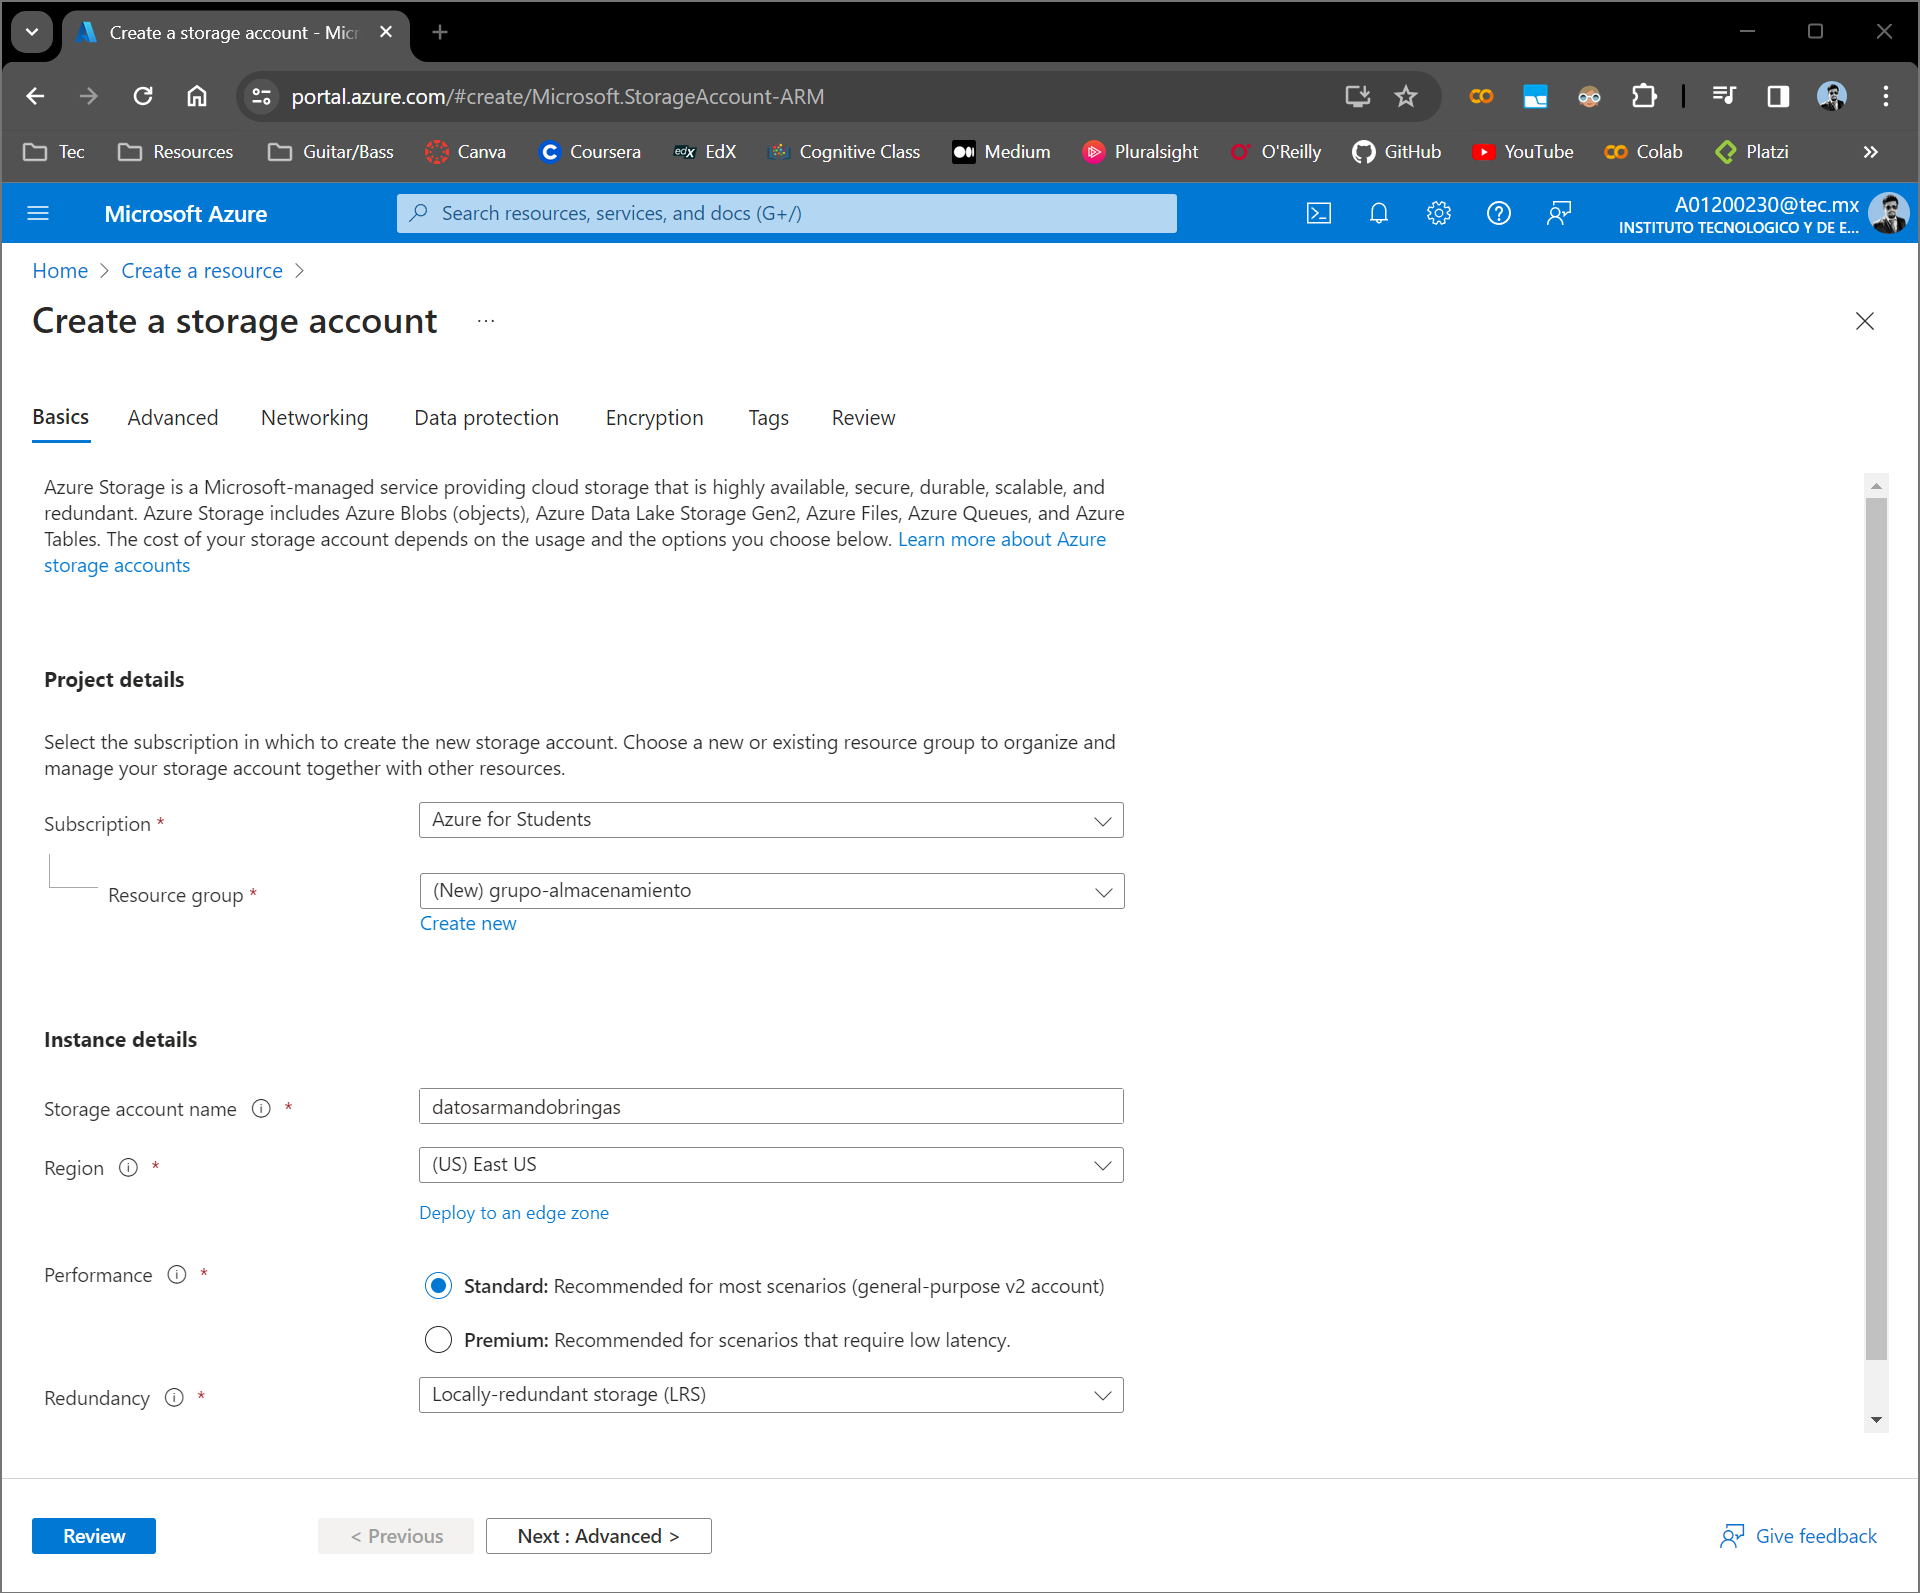
\includegraphics[width=1\linewidth]{M4_Servicios_Cómputo_en_la_Nube/Tarea_4_Crear_contenedores_en_la_nube/reporte/1-0_Creación_cuenta_storage.png}
    \captionof{lstlisting}{Creación de cuenta Azure Storage}
    \label{fig:Azure_0}
\end{figure}

En la siguiente figura \ref{fig:Azure_1} podemos observar que la cuenta quedó correctamente implementada con la creación de recursos, configuración de red y parámetros para posteriormente realizar la creación de nuestro contenedor.

\begin{figure}[H]
    \centering
    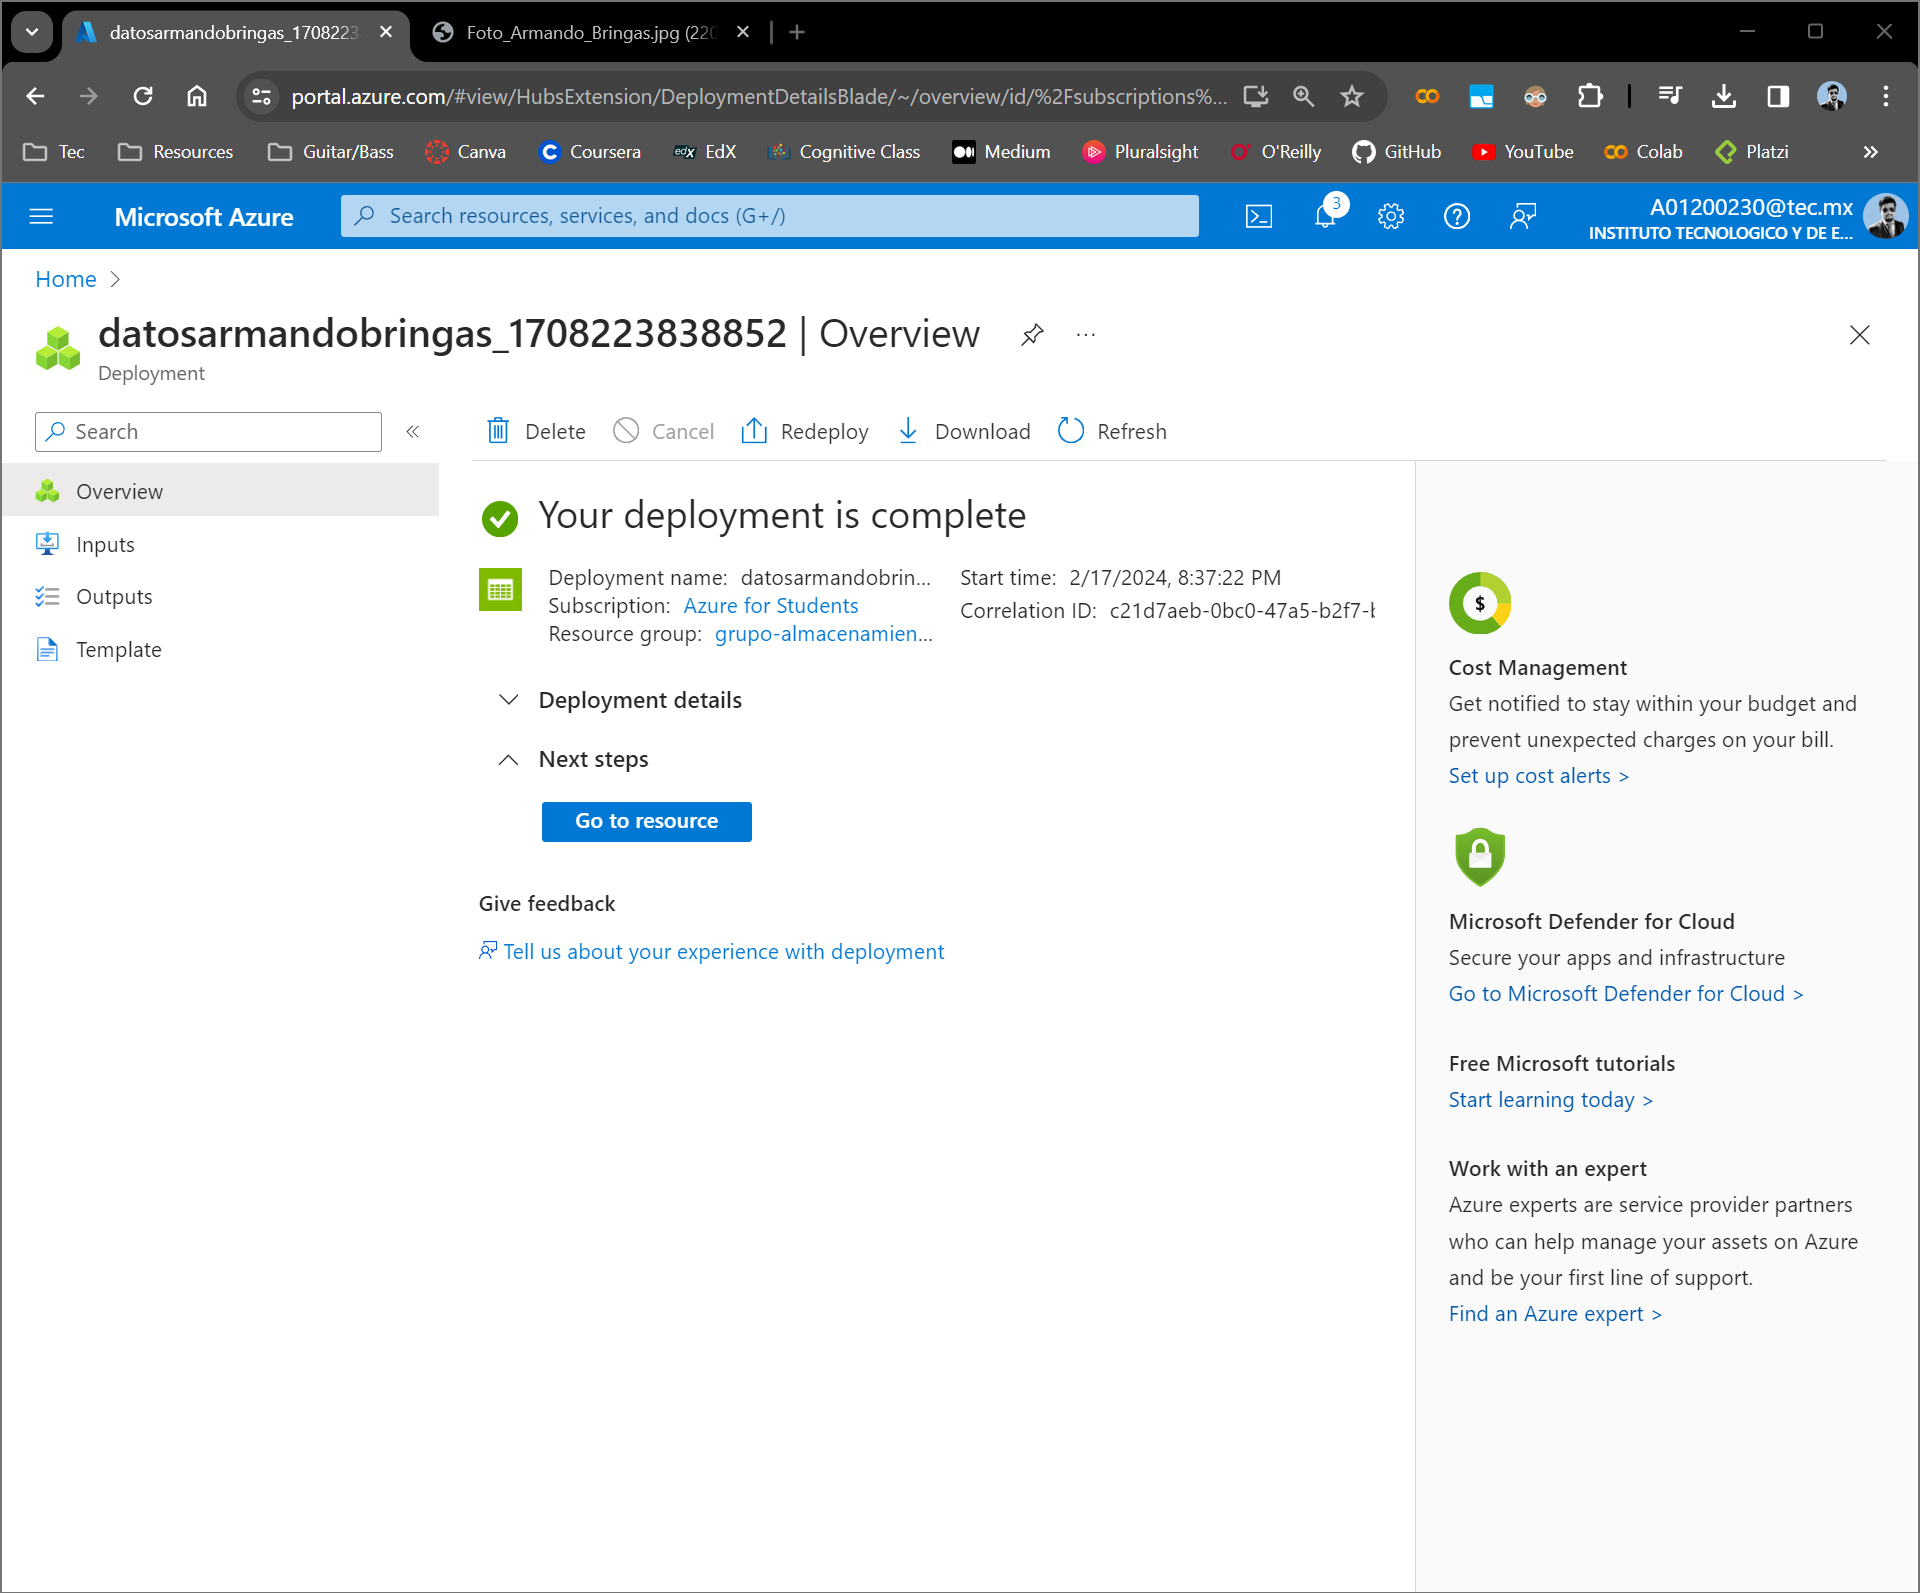
\includegraphics[width=1\linewidth]{M4_Servicios_Cómputo_en_la_Nube/Tarea_4_Crear_contenedores_en_la_nube/reporte/1-1_Creación_cuenta_storage.png.png}
    \captionof{lstlisting}{Implementación de cuenta Azure Storage}
    \label{fig:Azure_1}
\end{figure}

\vspace{3cm}

\subsection{Creación del contenedor Azure}

La siguiente figura \ref{fig:Azure_2} muestra la creación del contenedor \textbf{misdatos} en el cuál almacenaremos nuestra imagen y tendrá un nivel de acceso público.

\begin{figure}[H]
    \centering
    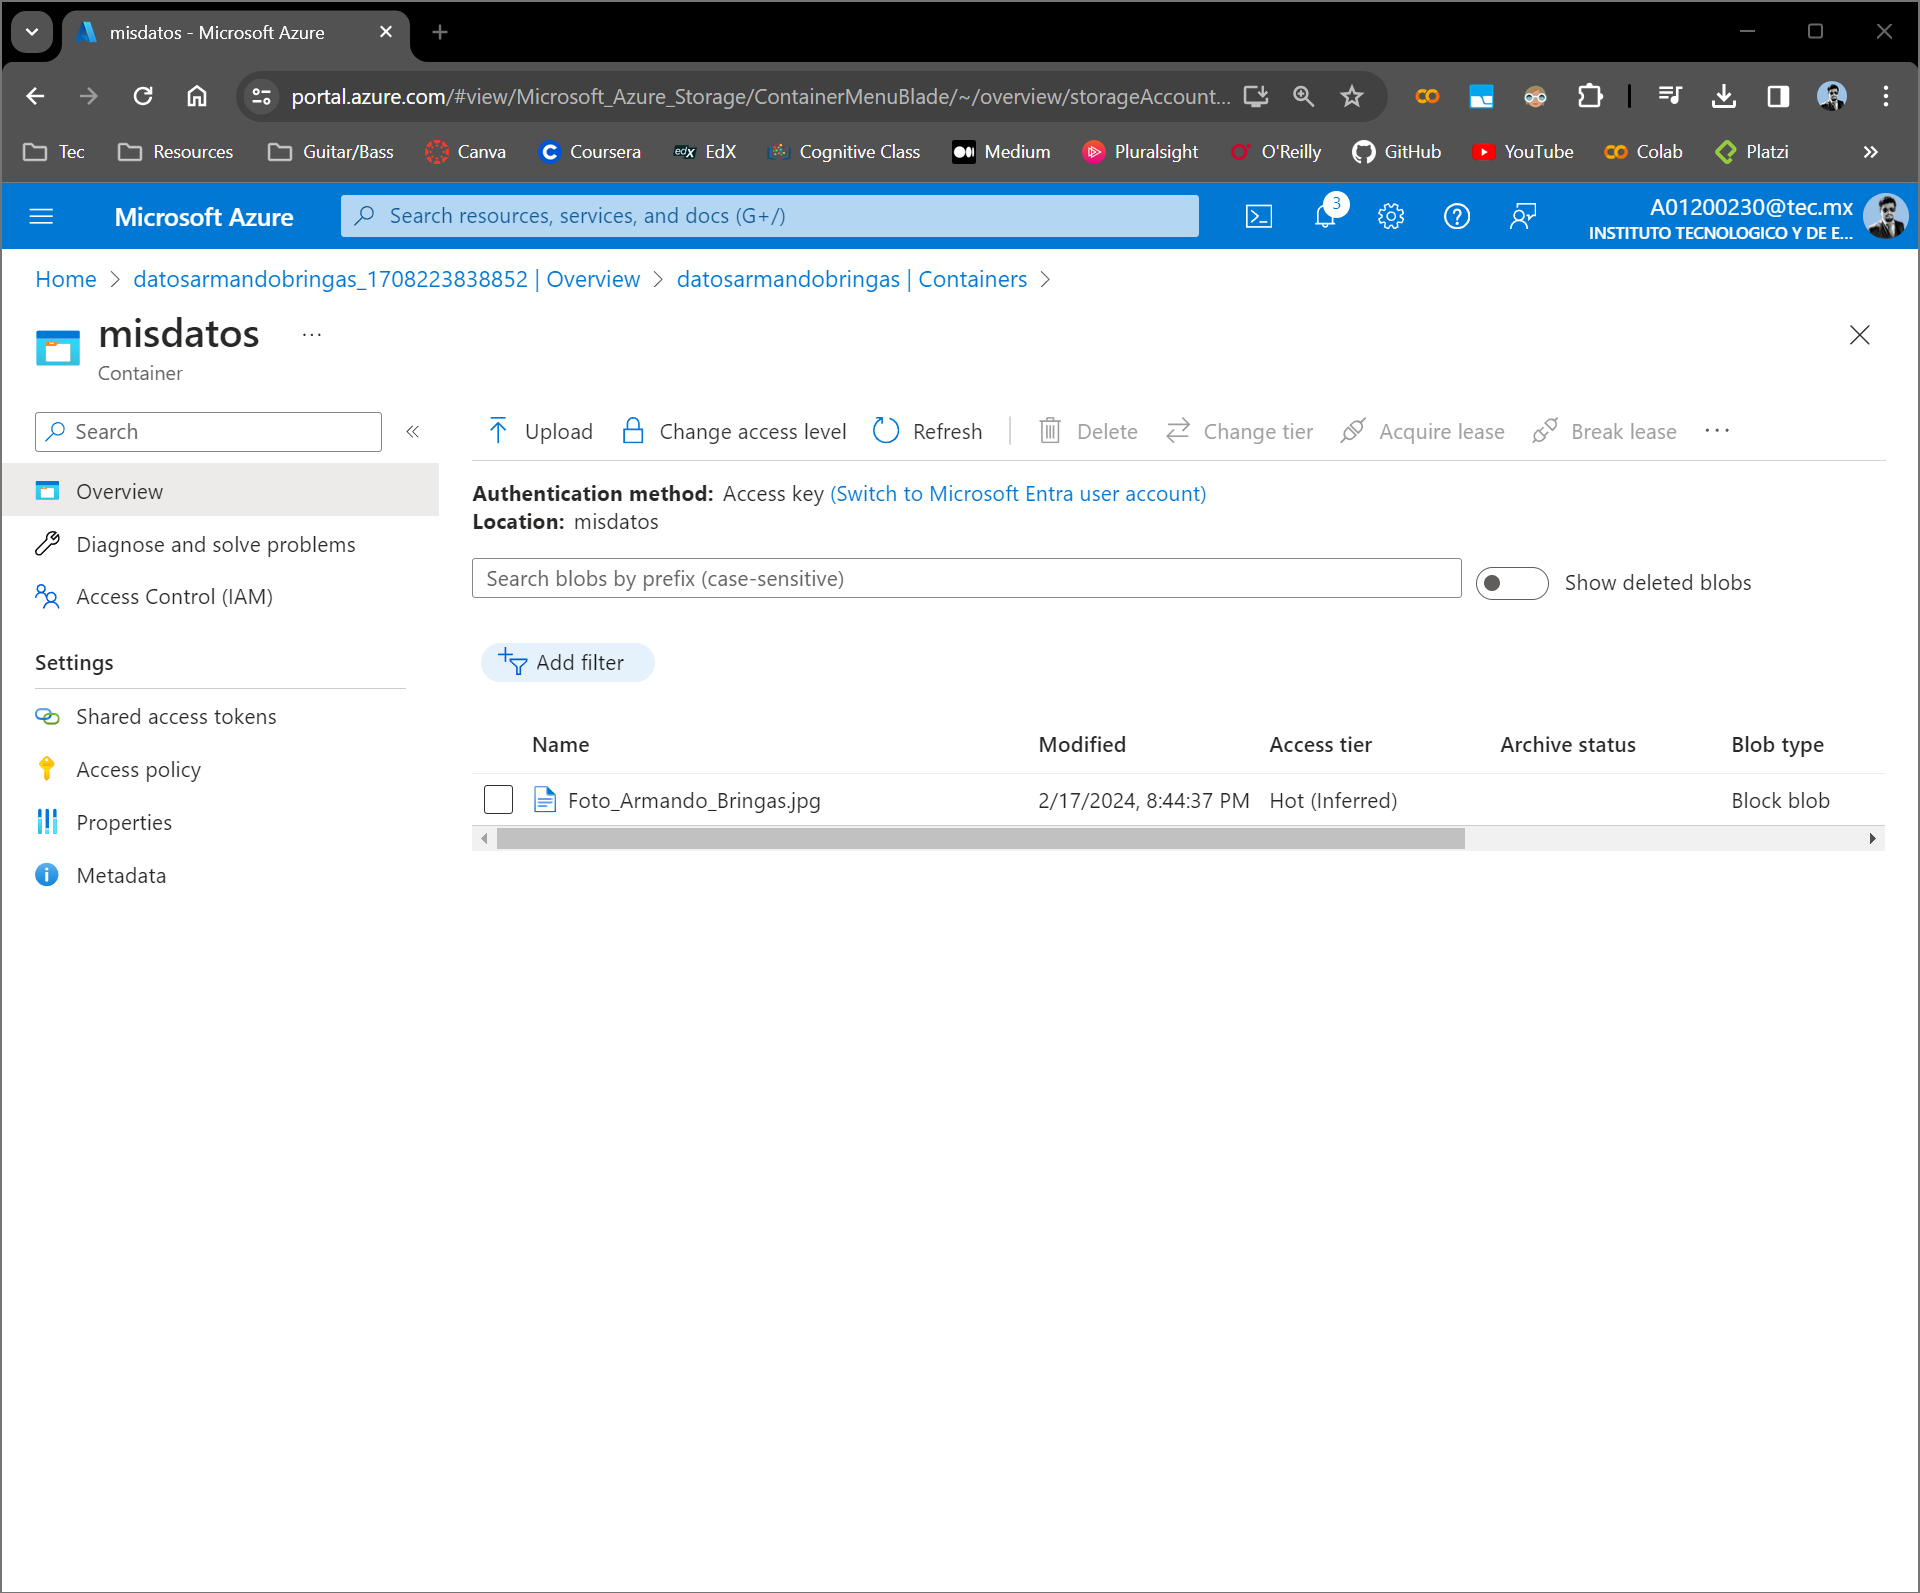
\includegraphics[width=1\linewidth]{M4_Servicios_Cómputo_en_la_Nube/Tarea_4_Crear_contenedores_en_la_nube/reporte/1-2_Creación_contenedor.png}
    \captionof{lstlisting}{Creación del contenedor en Azure}
    \label{fig:Azure_2}
\end{figure}

\vspace{3cm}

\subsection{Configuración del contenedor para que sea público}

A continuación en la figura \ref{fig:Azure_3} se observa que el contenedor fue configurado con un nivel de acceso público para que los archivos en el contenedor puedan accederse a través de internet.

\begin{figure}[H]
    \centering
    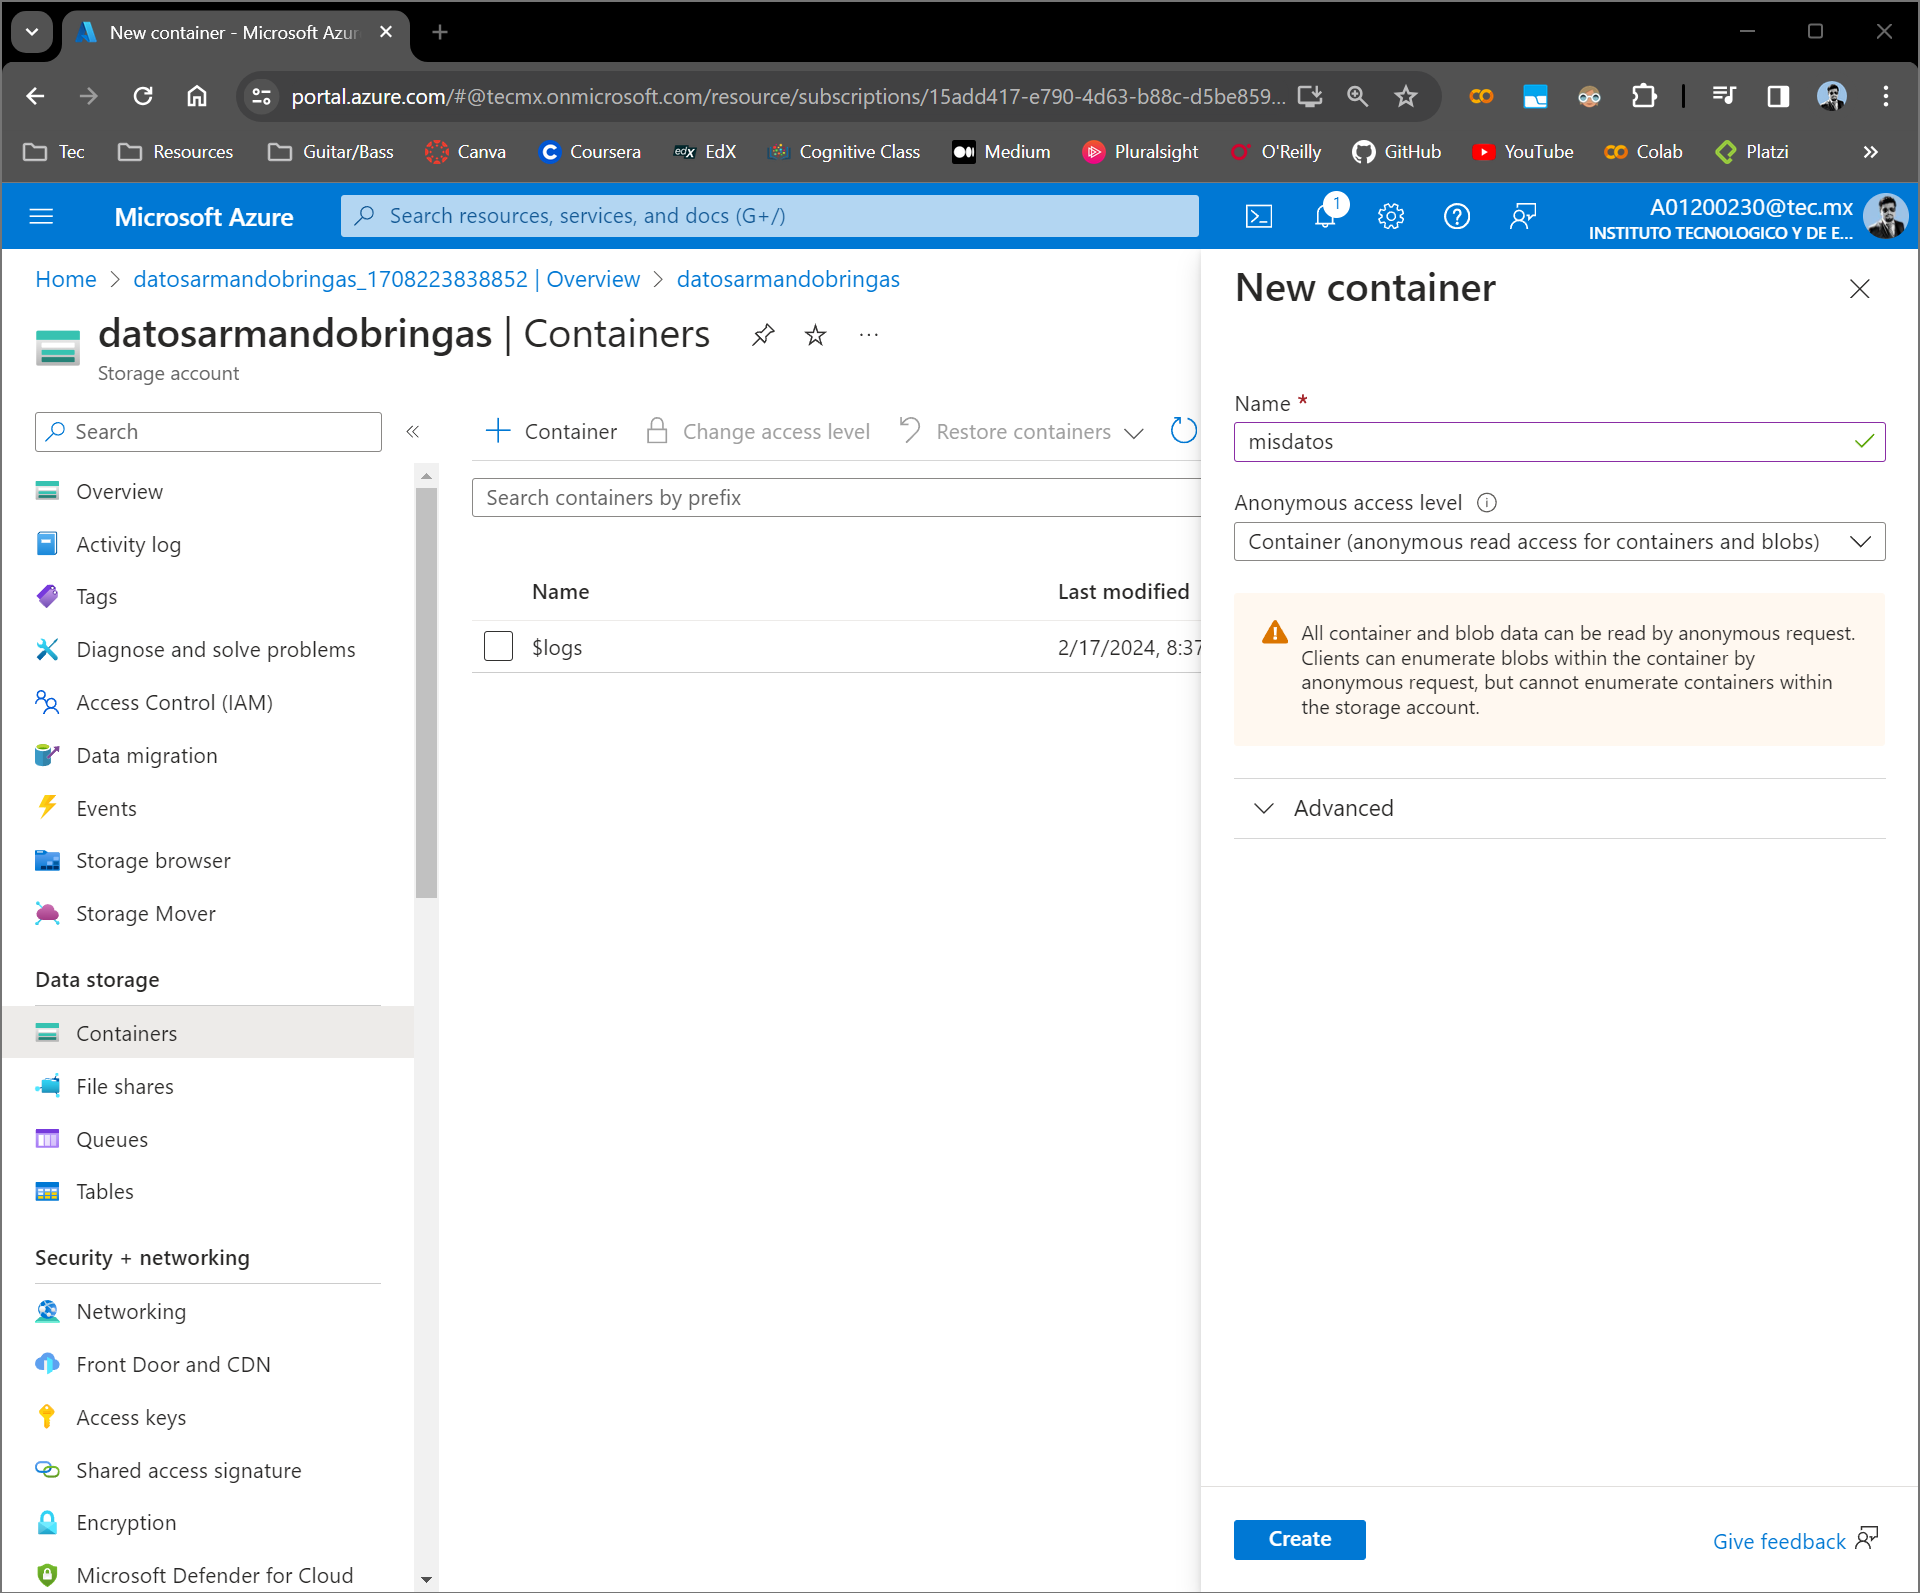
\includegraphics[width=1\linewidth]{M4_Servicios_Cómputo_en_la_Nube/Tarea_4_Crear_contenedores_en_la_nube/reporte/1-3_Configuración_contenedor_público.png}
    \captionof{lstlisting}{Configuración de acceso público al contenedor}
    \label{fig:Azure_3}
\end{figure}

\vspace{3cm}

\subsection{Carga de los archivos}

Posteriormente se procede al cargado de la imagen que se va a cargar en el contenedor y obtenemos la dirección URL para poder acceder a la visualización de la imagen desde cualquier navegador.

\begin{figure}[H]
    \centering
    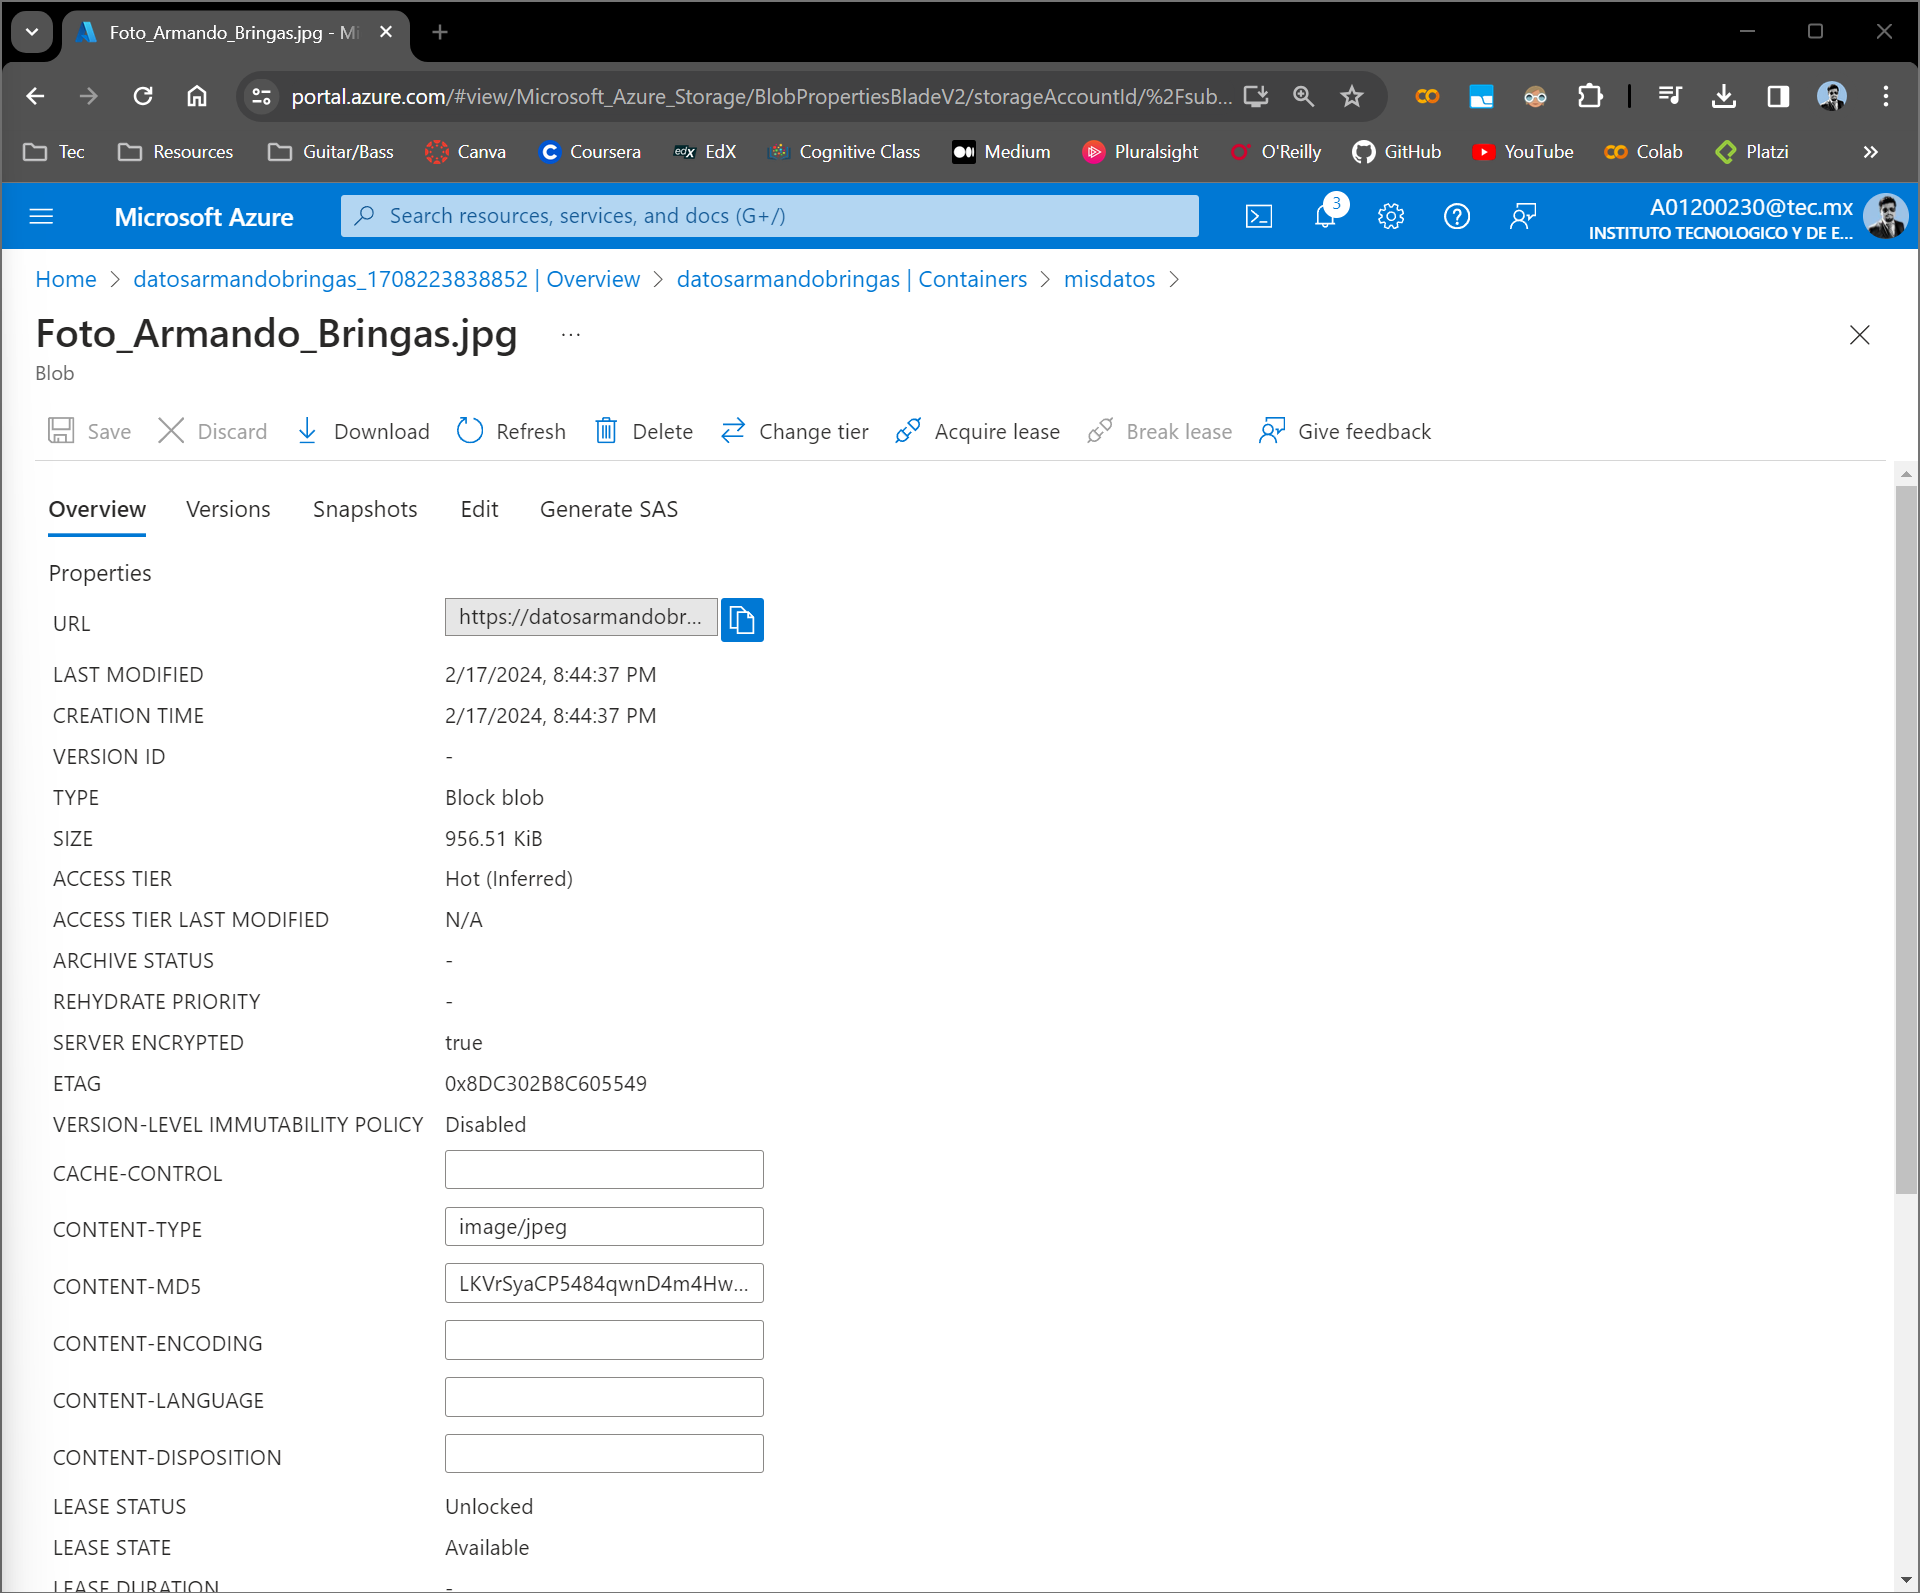
\includegraphics[width=1\linewidth]{M4_Servicios_Cómputo_en_la_Nube/Tarea_4_Crear_contenedores_en_la_nube/reporte/1-4_Carga_archivo.png}
    \captionof{lstlisting}{Cargado de archivo en el contenedor}
    \label{fig:Azure_4}
\end{figure}

\vspace{5cm}

En la siguiente figura \ref{fig:Azure_5} se muestra la carga de la imagen a través de la URL \url{https://datosarmandobringas.blob.core.windows.net/misdatos/Foto_Armando_Bringas.jpg}

\begin{figure}[H]
    \centering
    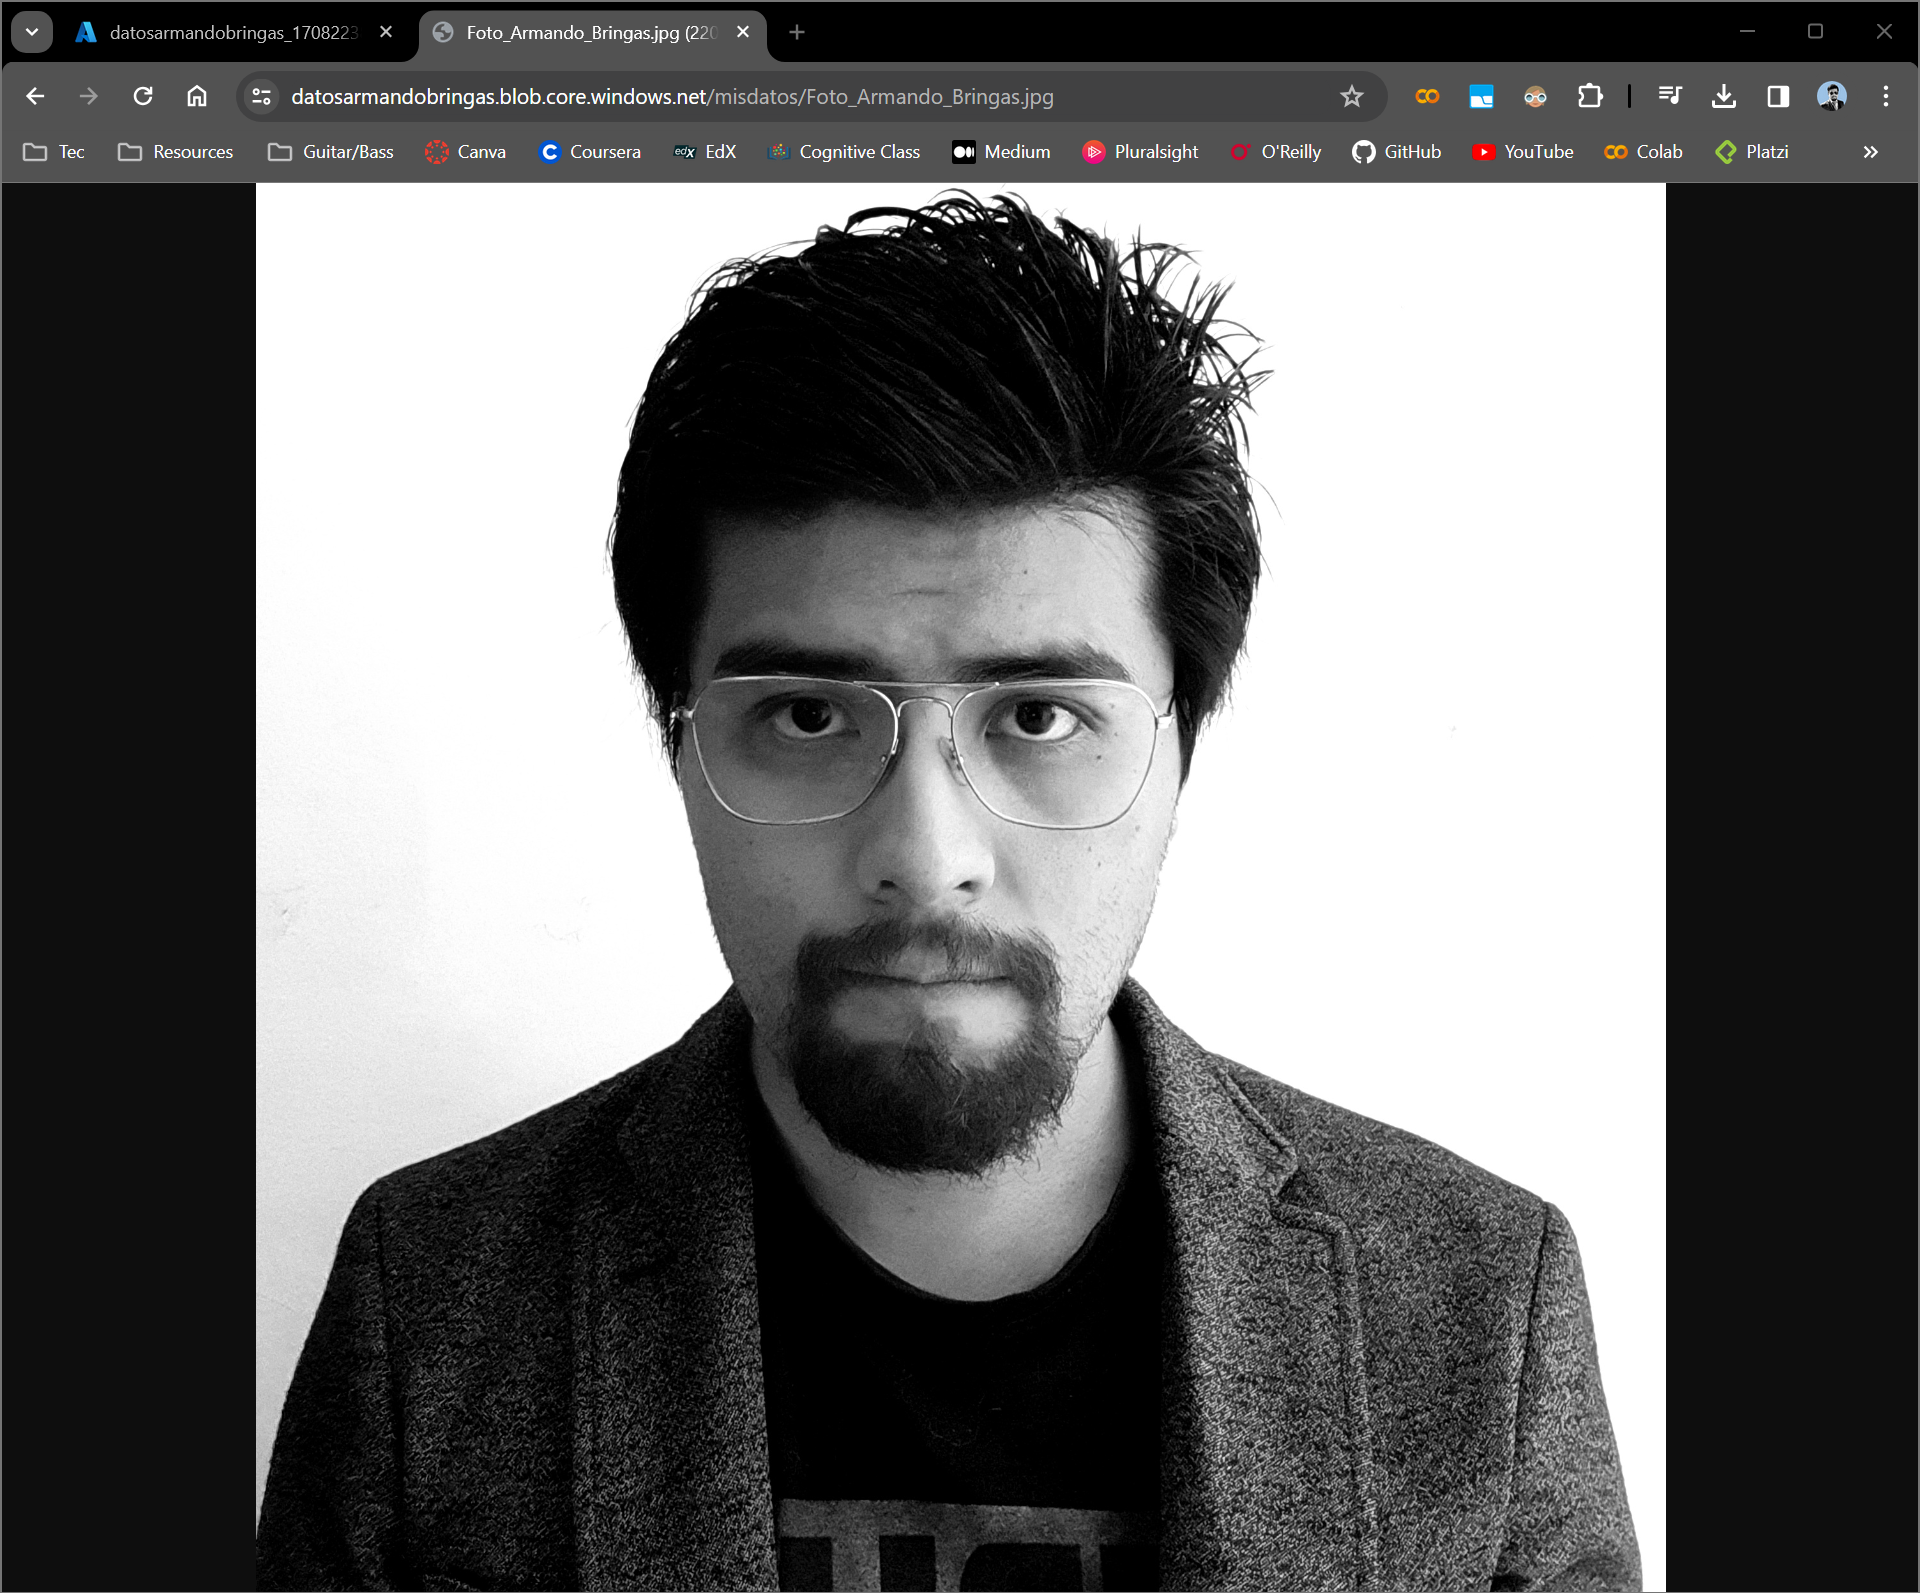
\includegraphics[width=1\linewidth]{M4_Servicios_Cómputo_en_la_Nube/Tarea_4_Crear_contenedores_en_la_nube/reporte/1-5_Carga_archivo.png}
    \captionof{lstlisting}{Visualización de imagen del contenedor}
    \label{fig:Azure_5}
\end{figure}

\vspace{5cm}

\section{Contenedor Google}

Para poder crear nuestro contenedor de Google lo hacemos a través de la consola de \textit{Cloud Skills Boost} donde cargamos una actividad que nos diera oportunidad de de crear un \textbf{Bucket} (Contenedor en Google Cloud).

\begin{figure}[H]
    \centering
    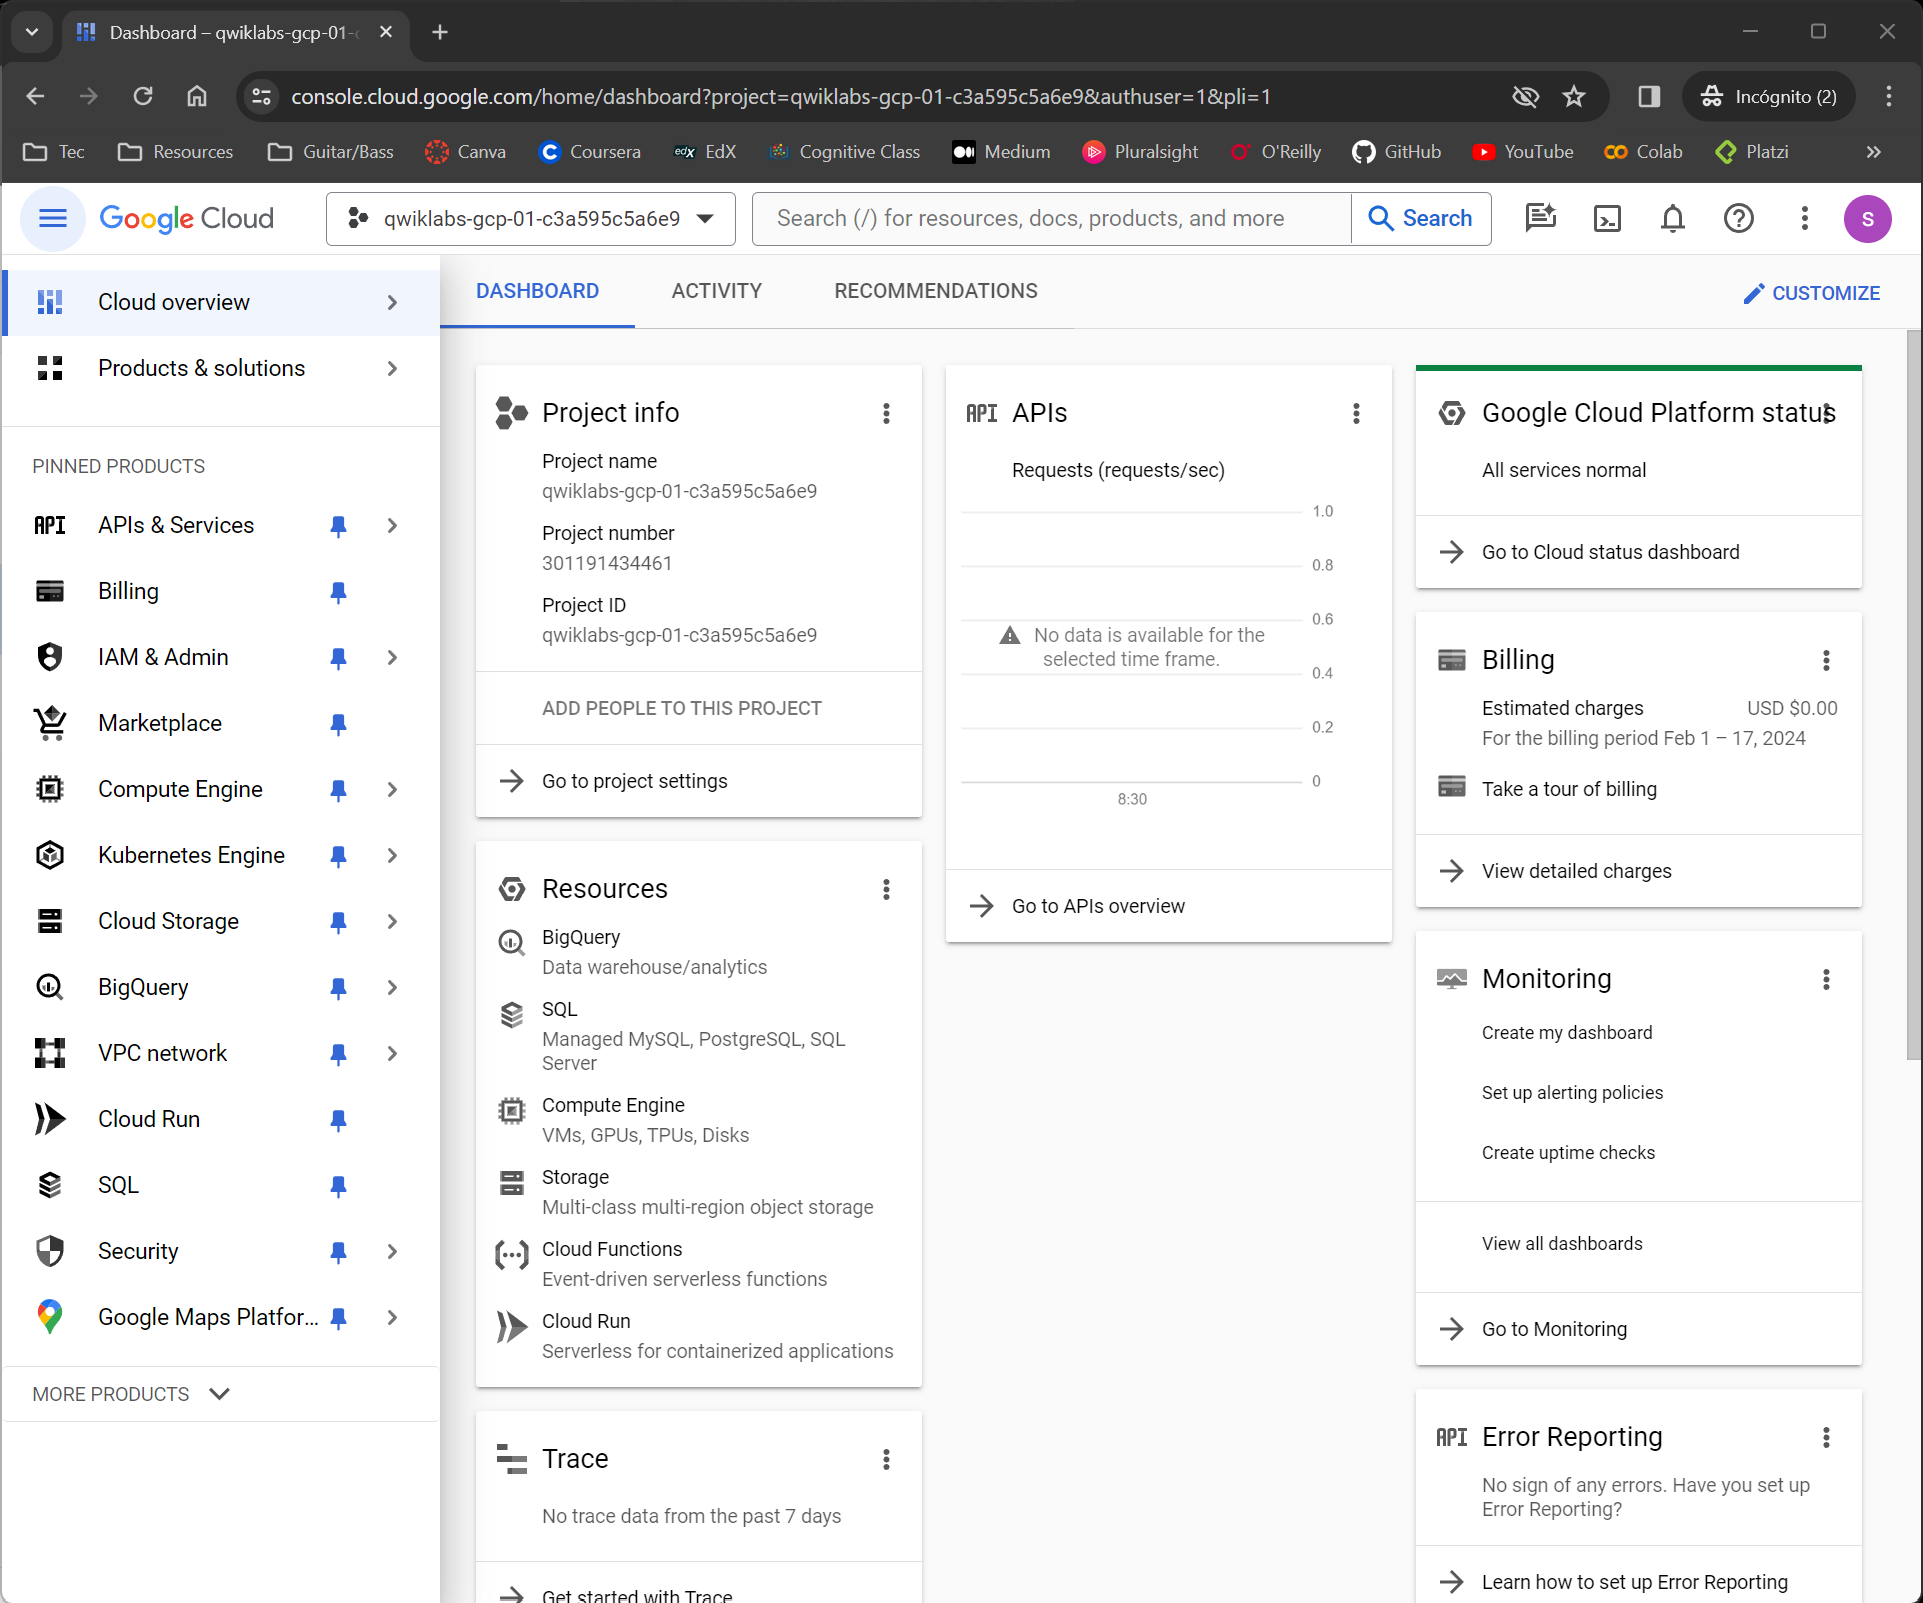
\includegraphics[width=1\linewidth]{M4_Servicios_Cómputo_en_la_Nube/Tarea_4_Crear_contenedores_en_la_nube/reporte/2-0_Acceso_Laboratorio_Google.png}
    \captionof{lstlisting}{Acceso al laboratorio de Google Cloud}
    \label{fig:Google_0}
\end{figure}

\vspace{5cm}

\subsection{Creación del contenedor Google}

Accedemos a través de la consola a \textbf{Cloud Storage} donde creamos el Bucket donde nos aseguramos que la opción de \textit{Enforce public access prevention on this bucket} no esté marcada para poder permitir el acceso a la visualización de la imagen que se estará cargando.

\begin{figure}[H]
    \centering
    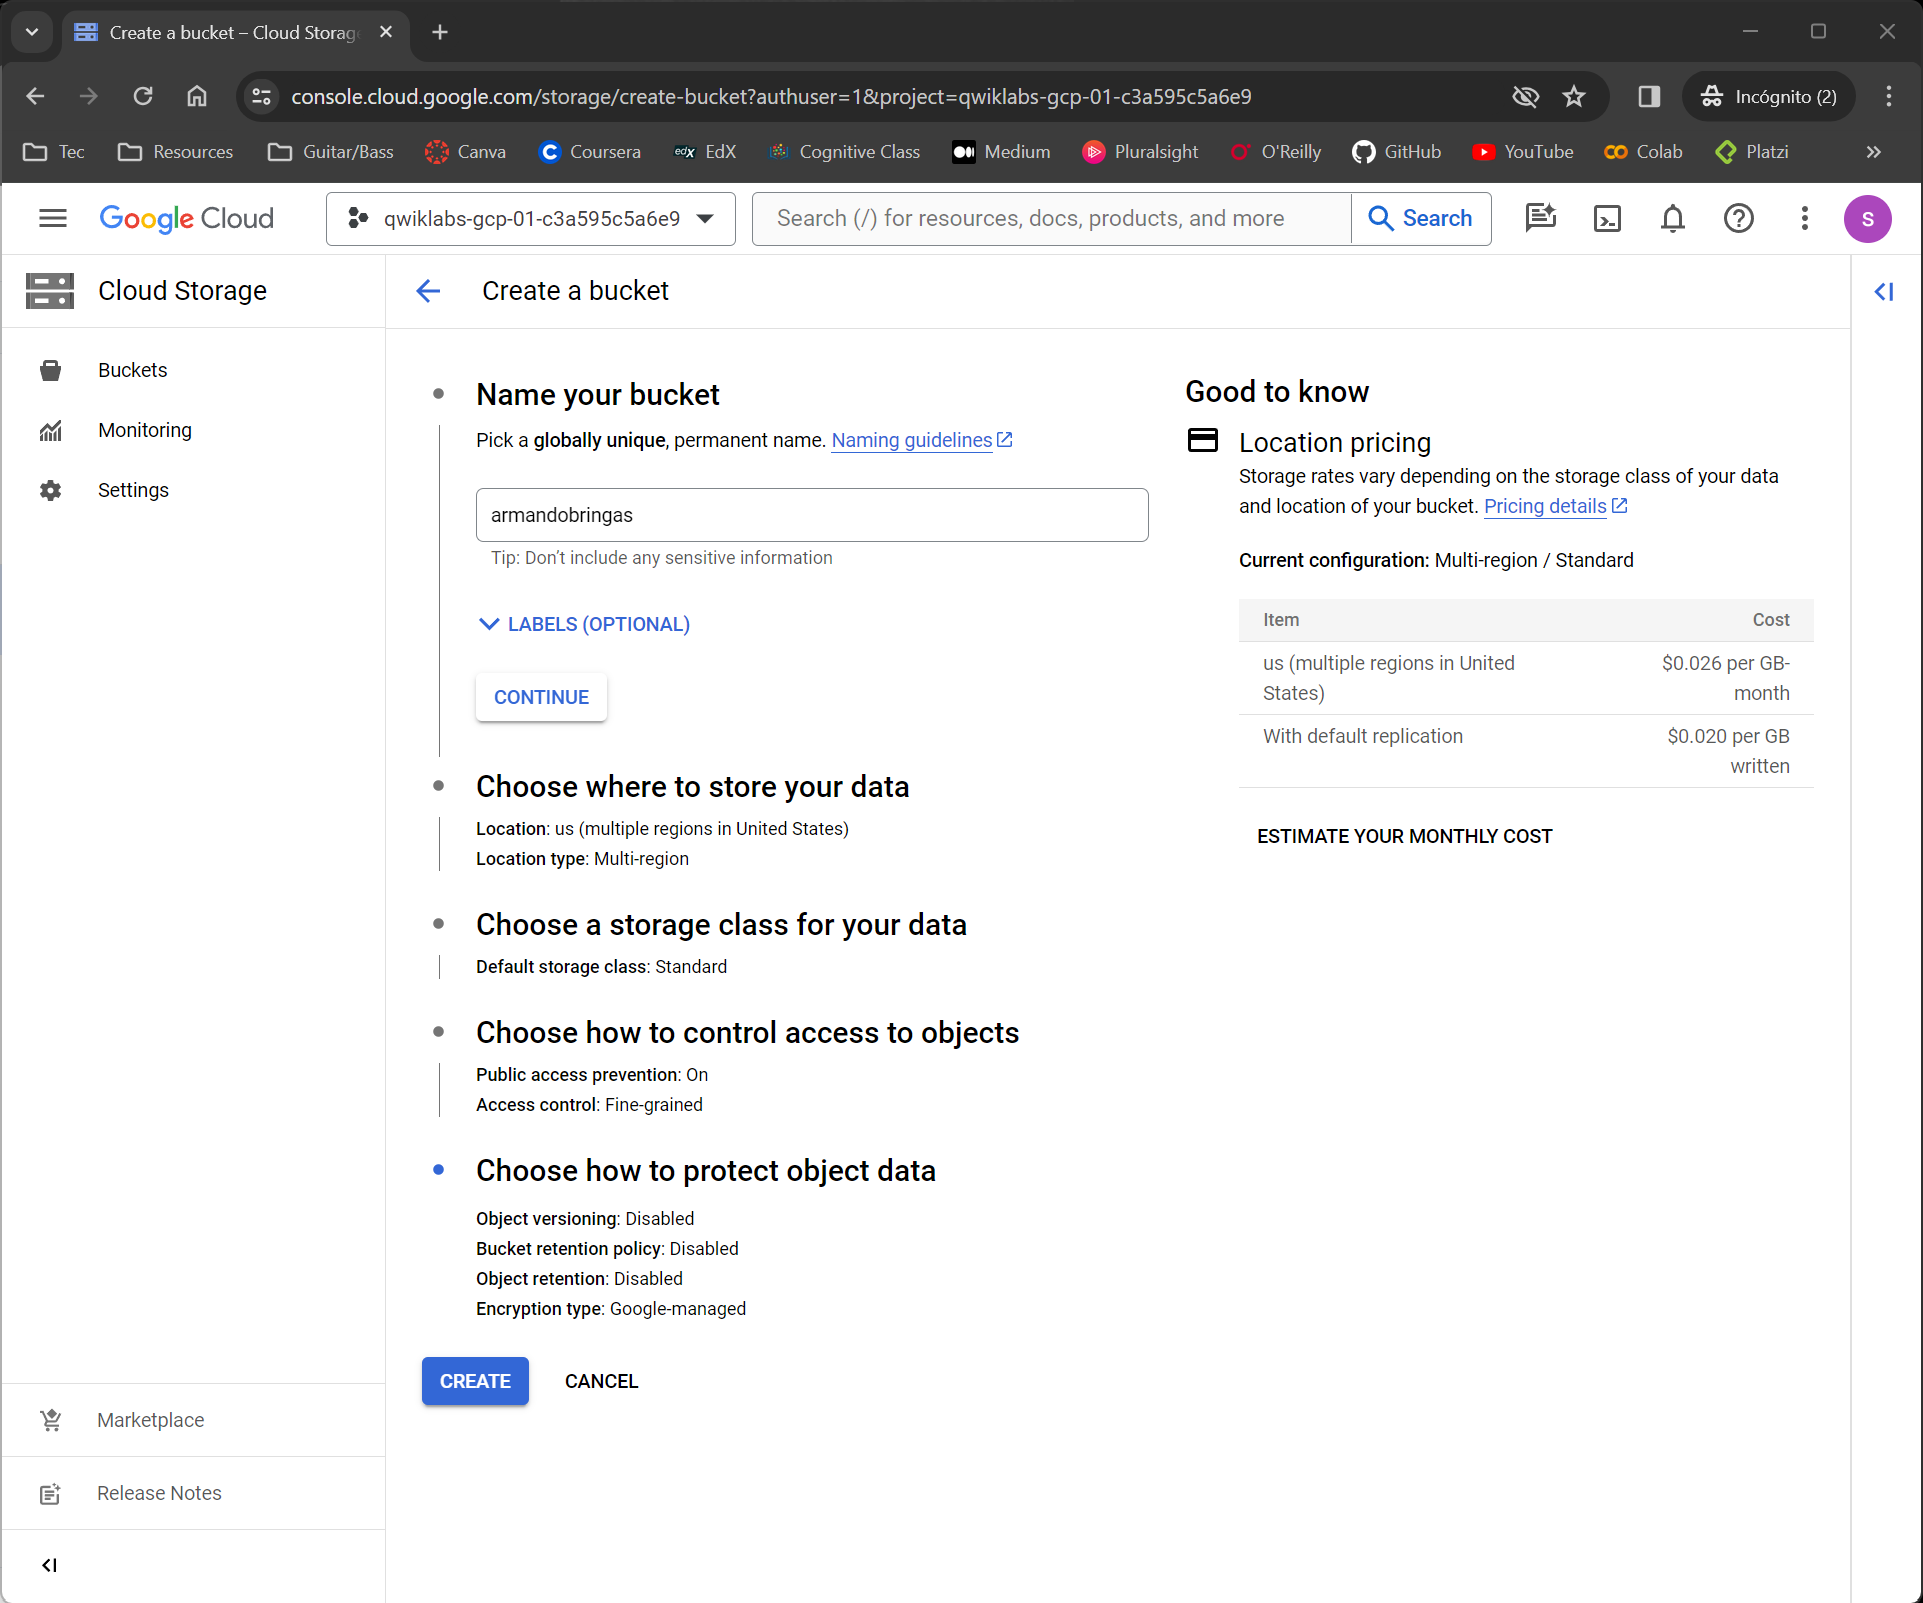
\includegraphics[width=1\linewidth]{M4_Servicios_Cómputo_en_la_Nube/Tarea_4_Crear_contenedores_en_la_nube/reporte/2-1_Creación_contenedor.png}
    \captionof{lstlisting}{Creación del contenedor en Google Cloud}
    \label{fig:Google_1}
\end{figure}

\vspace{5cm}

\subsection{Configuración del contenedor para que sea público}

Previamente ya habíamos hecho la carga del archivo como se mostrará en la siguiente sección, sin embargo, como se muestra en la figura \ref{fig:Google_2}, se cambió el último registro para permitir el acceso público de lectura al archivo para que se pueda accesar a través de Intenet.

\begin{figure}[H]
    \centering
    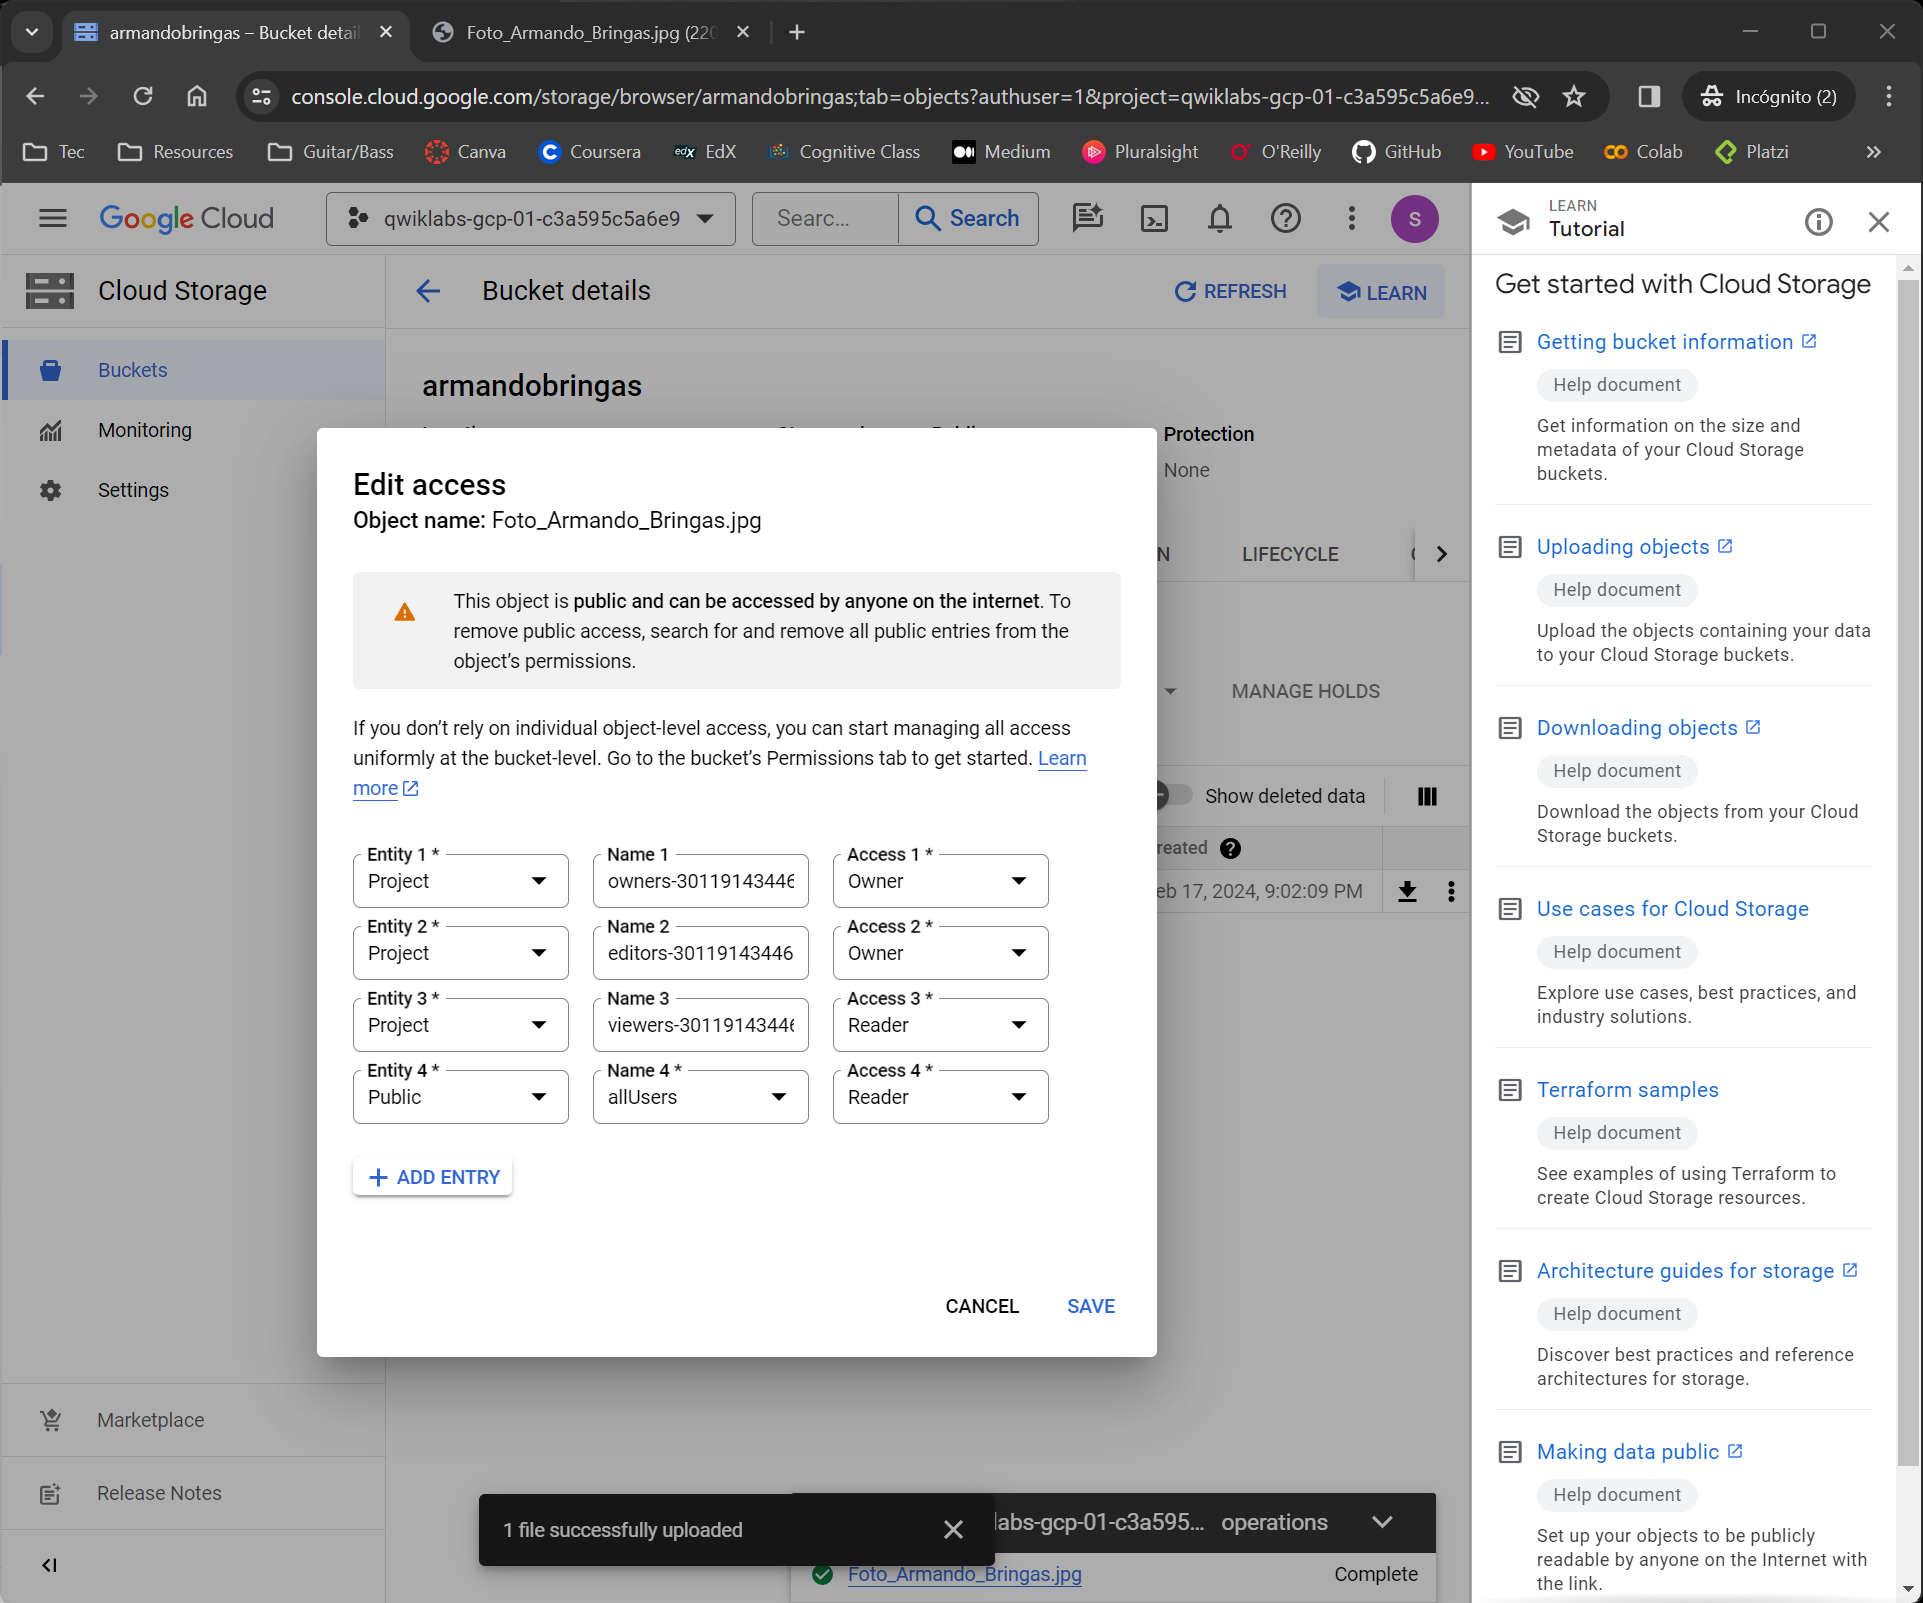
\includegraphics[width=1\linewidth]{M4_Servicios_Cómputo_en_la_Nube/Tarea_4_Crear_contenedores_en_la_nube/reporte/2-2_Configuración_contenedor_público.png}
    \captionof{lstlisting}{Configuración de acceso público al contenedor}
    \label{fig:Google_2}
\end{figure}

\vspace{5cm}

\subsection{Carga de los archivos}

En la siguiente figura \ref{fig:Google_3} se observa el cargado de la imagen en el contenedor. En la figura \ref{fig:Google_4} se observa que se obtiene una URL autentificada la cual nos permite tener acceso a la visualización del archivo desde cualquier navegador.

\begin{figure}[H]
    \centering
    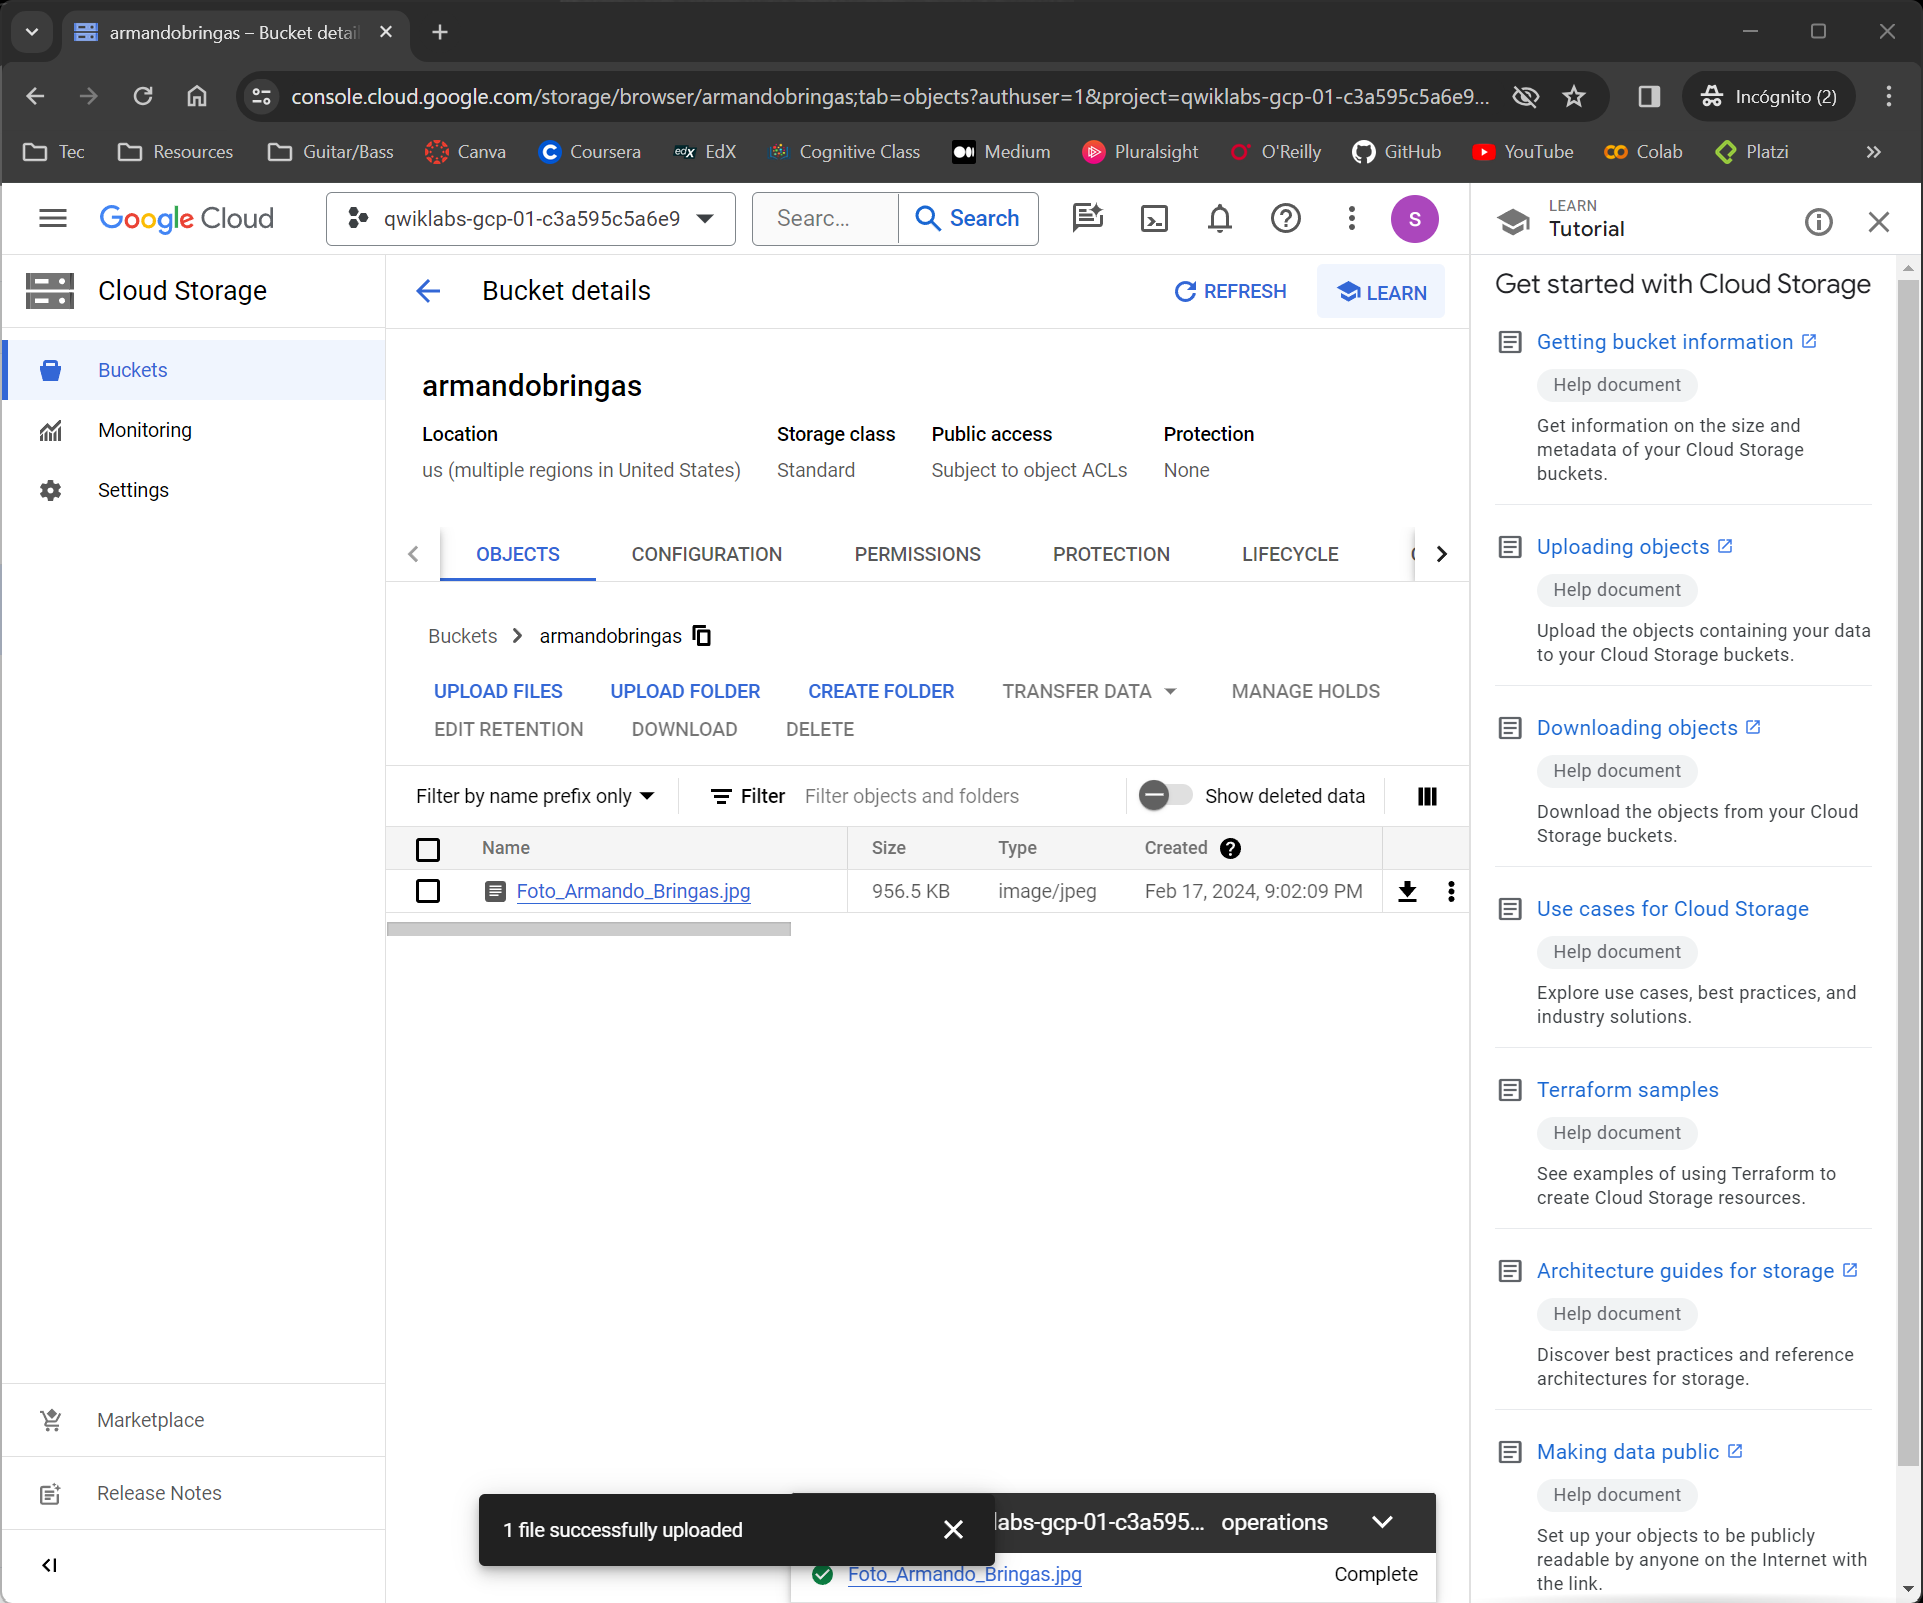
\includegraphics[width=1\linewidth]{M4_Servicios_Cómputo_en_la_Nube/Tarea_4_Crear_contenedores_en_la_nube/reporte/2-3_Carga_archivo.png}
    \captionof{lstlisting}{Cargado de archivo en el contenedor}
    \label{fig:Google_3}
\end{figure}

\begin{figure}[H]
    \centering
    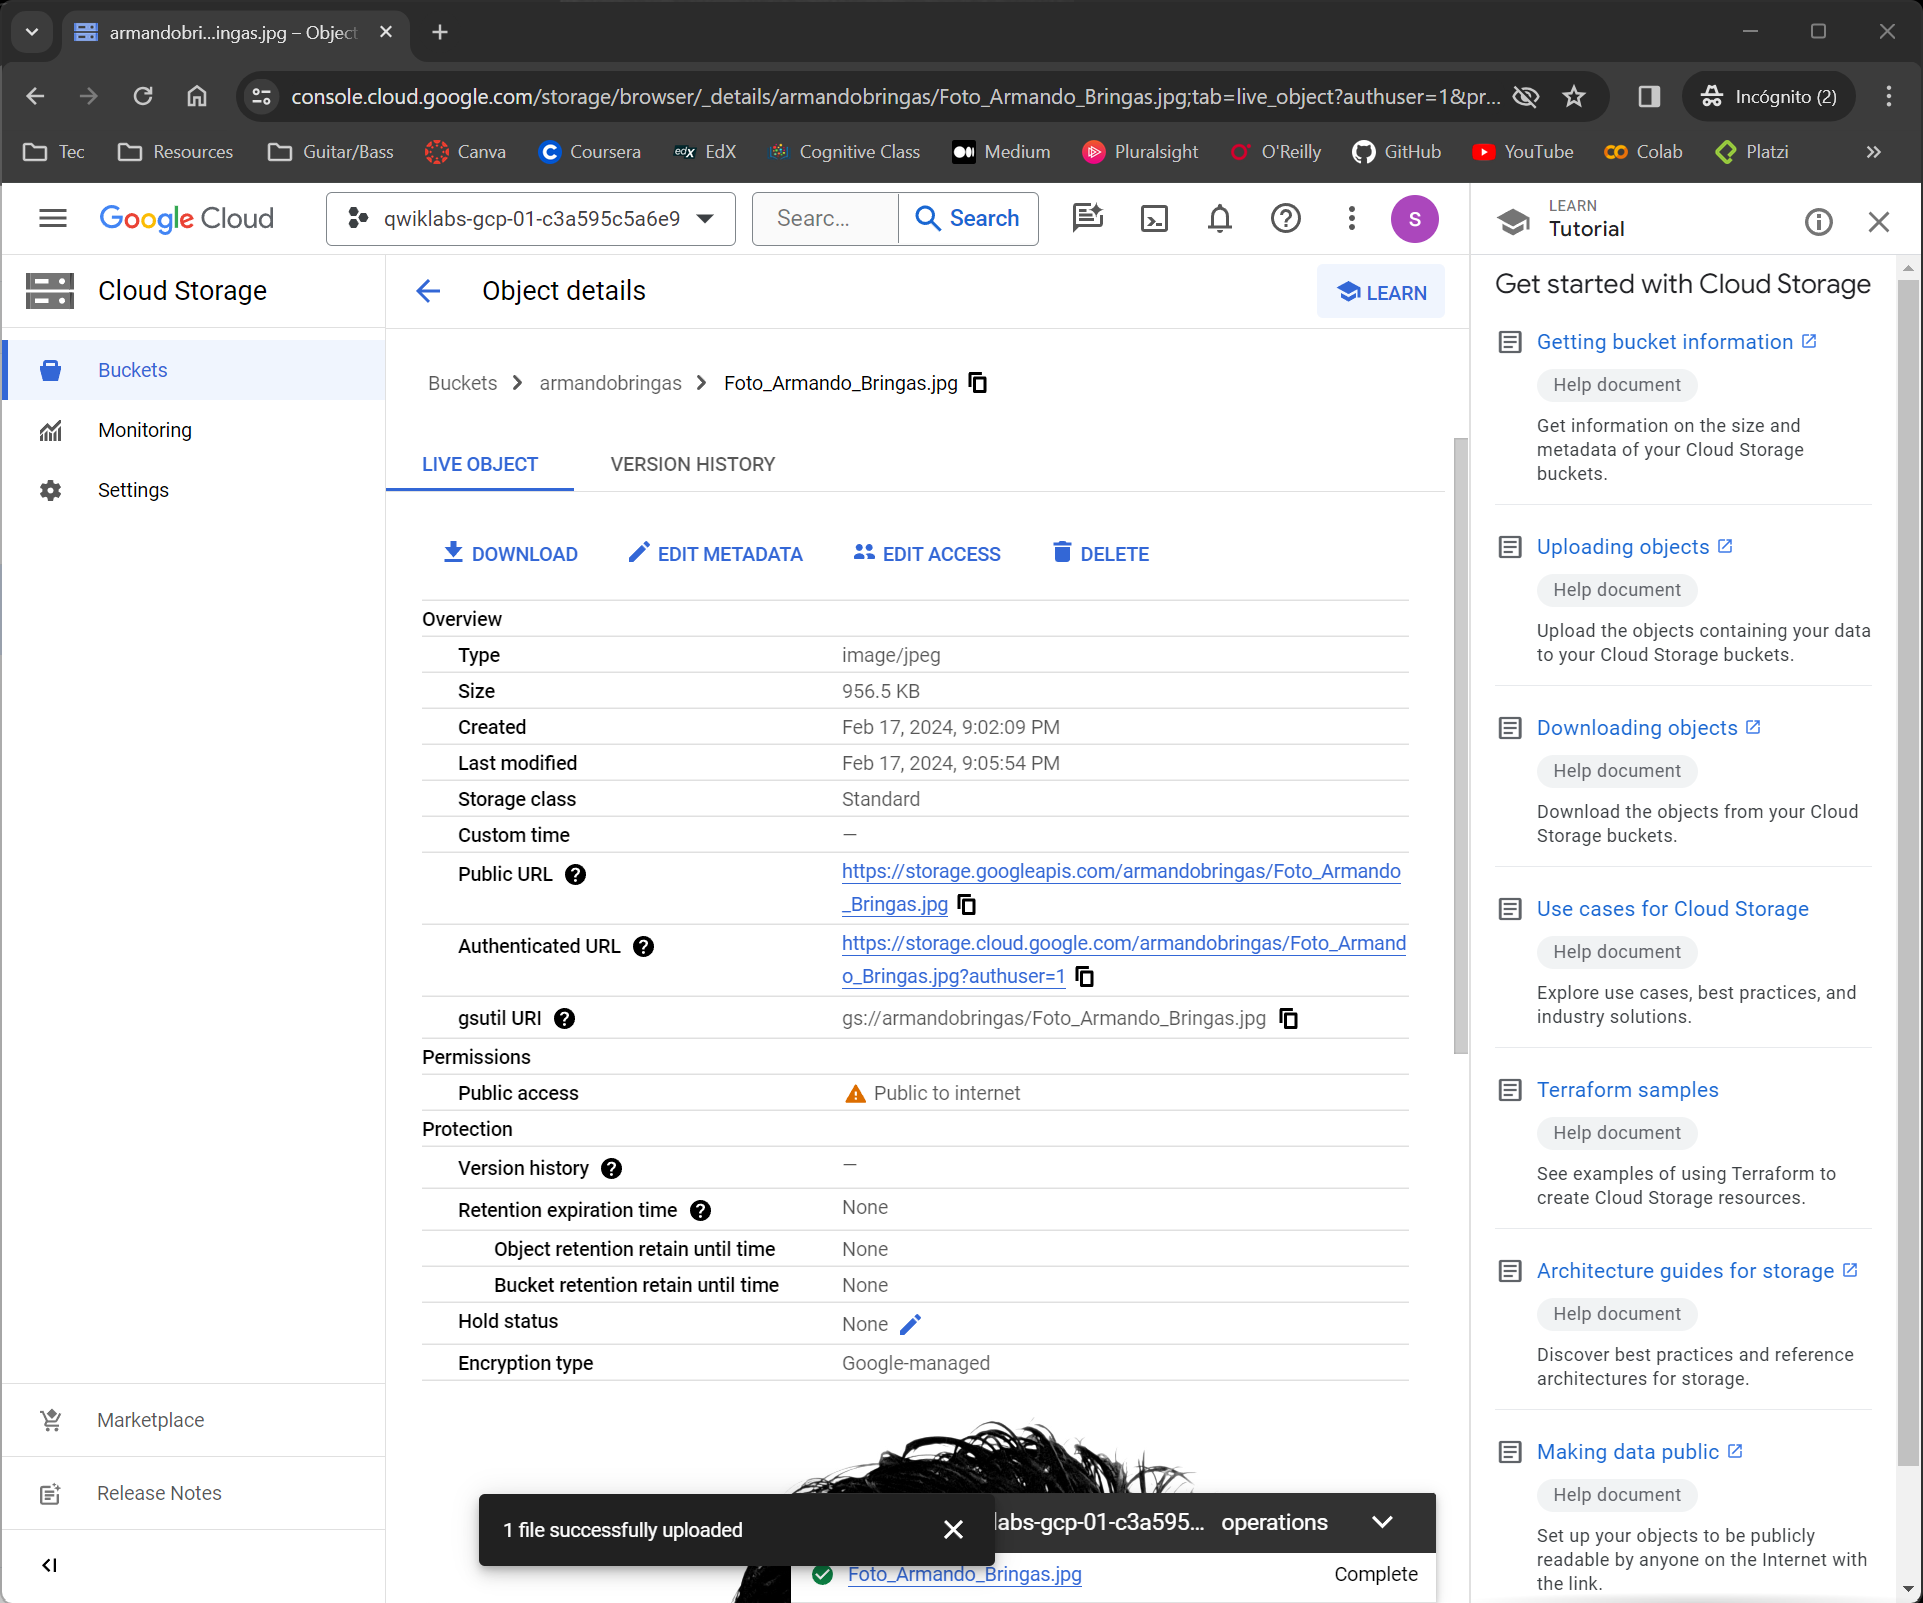
\includegraphics[width=1\linewidth]{M4_Servicios_Cómputo_en_la_Nube/Tarea_4_Crear_contenedores_en_la_nube/reporte/2-4_Carga_archivo.png}
    \captionof{lstlisting}{Obtención de URL autentificada}
    \label{fig:Google_4}
\end{figure}

\vspace{10cm}

Finalmente, como se observa en figura \ref{fig:Google_5} comprobamos que podemos visualizar nuestra imagen a través de la siguiente URL autentificada \url{https://storage.cloud.google.com/armandobringas/Foto_Armando_Bringas.jpg?authuser=1}. \textbf{En importante mencionar que la liga ya no funciona debido a que el recurso se elimino una vez que finalizamos el laboratorio.}

\begin{figure}[H]
    \centering
    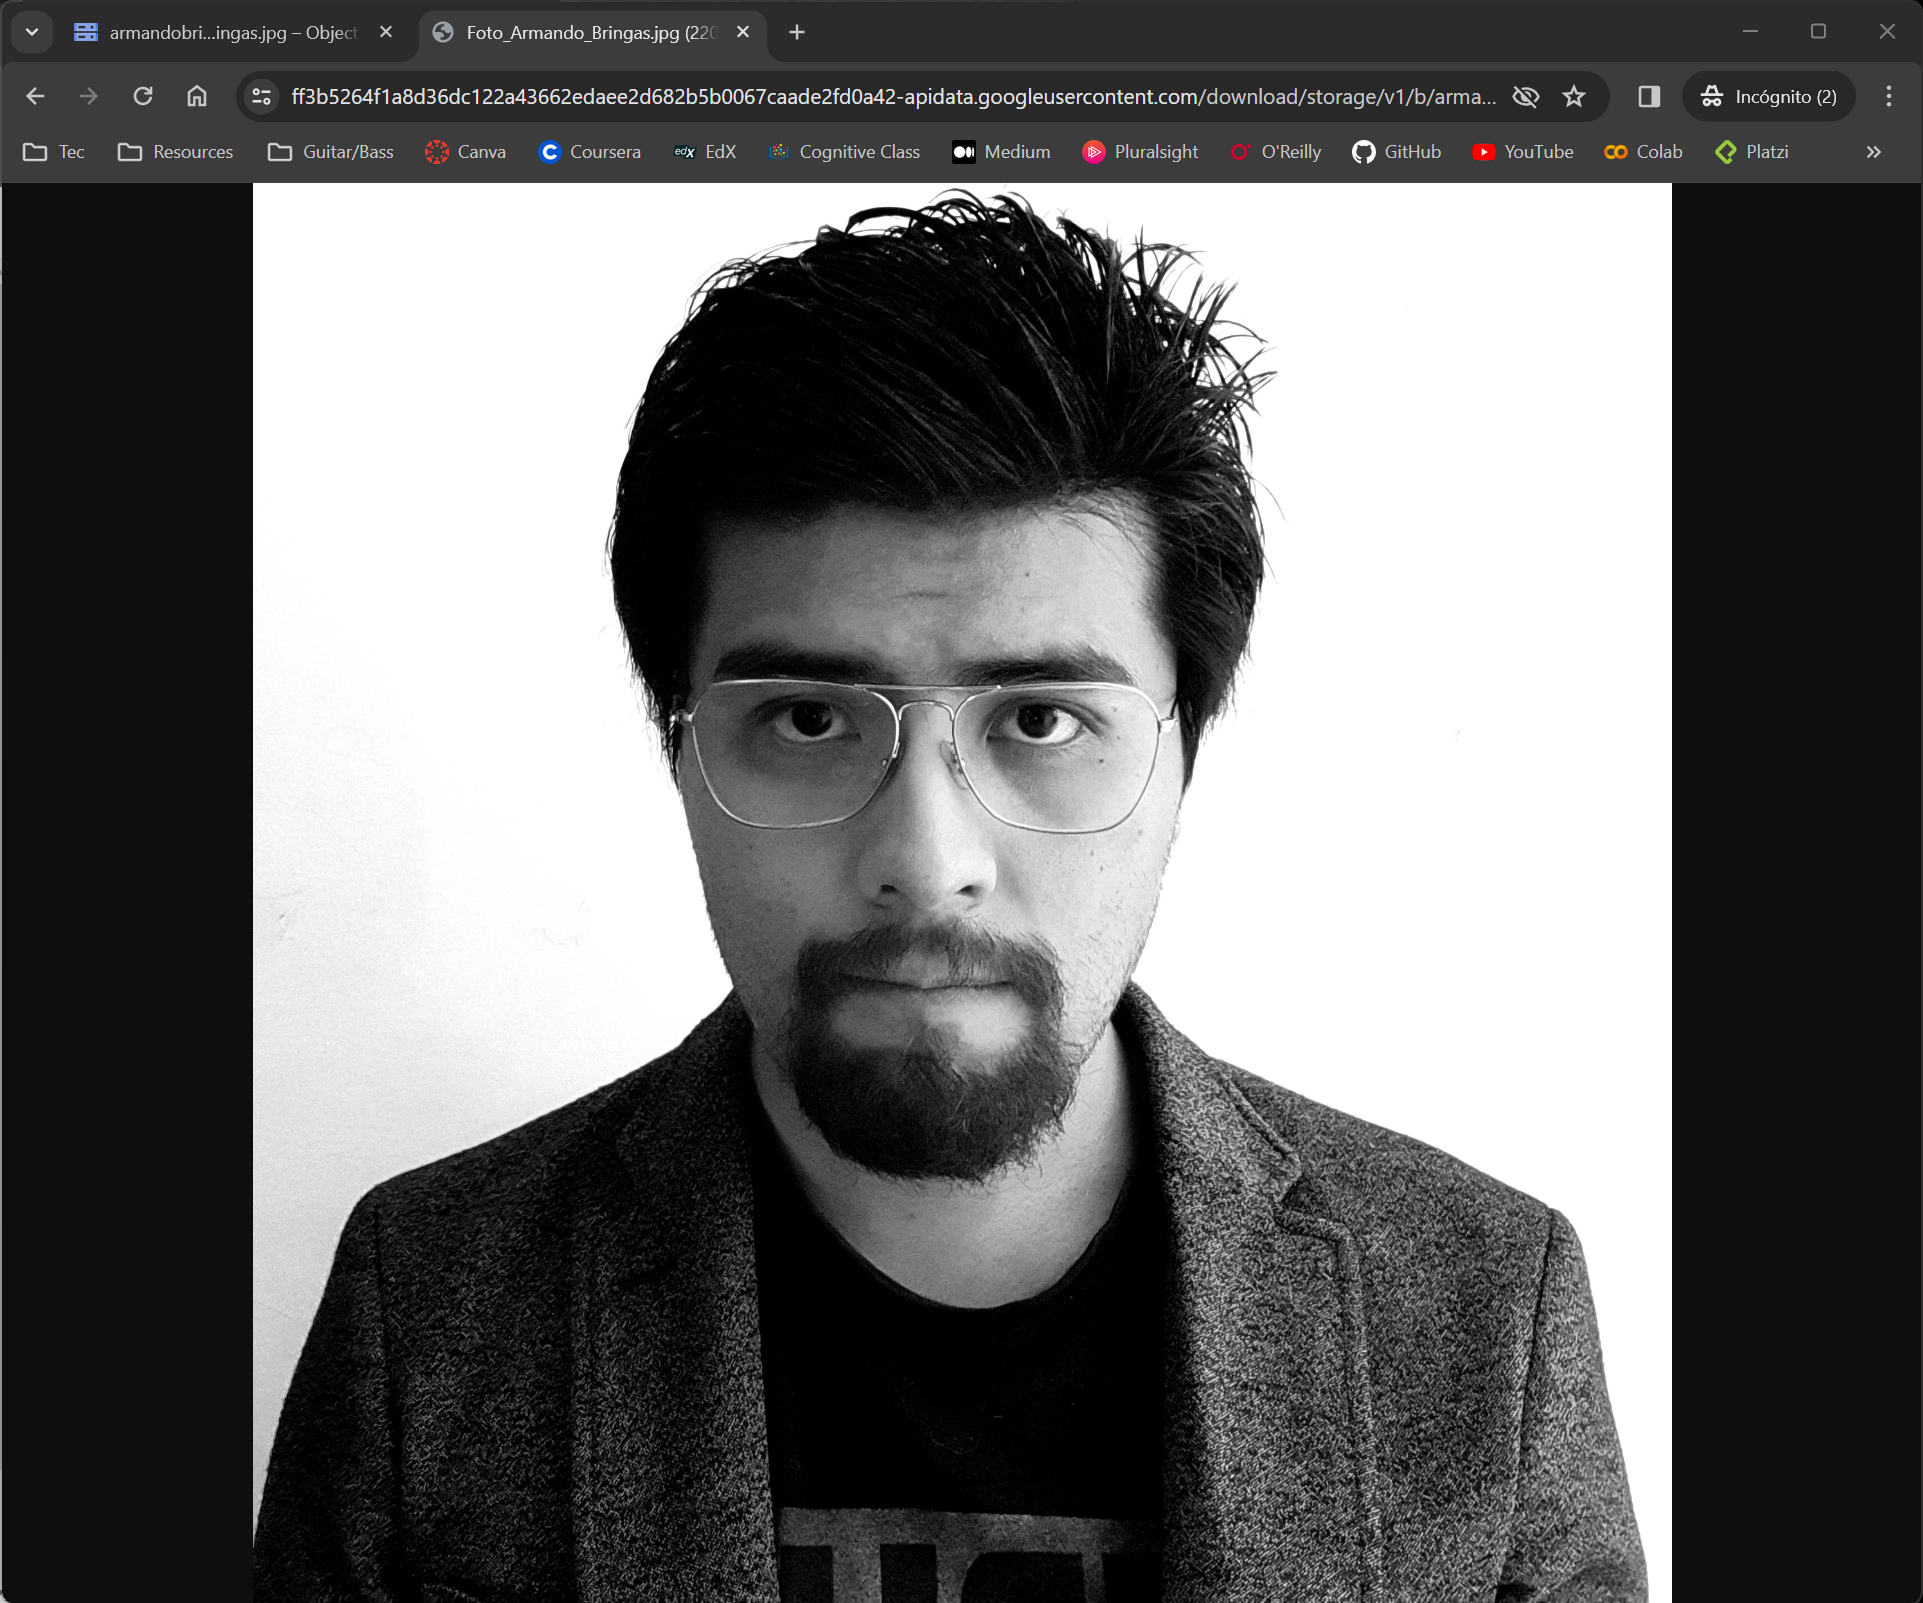
\includegraphics[width=1\linewidth]{M4_Servicios_Cómputo_en_la_Nube/Tarea_4_Crear_contenedores_en_la_nube/reporte/2-5_Carga_archivo.png}
    \captionof{lstlisting}{Visualización de imagen del contenedor}
    \label{fig:Google_5}
\end{figure}

\vspace{1em}

\end{document}